\section{Elettromagnetismo}\label{sec:2}
\subsection{Forza di Lorentz}\label{sec:2.1}
Alla luce di quanto detto alla fine della sezione \ref{sec:1.6} possiamo studiare la dinamica di una particella carica sottoposta ad un campo elettromagnetico. Dunque, nel caso considerato, il principio di inerzia \eqref{eq:princ_iner} e il teorema delle forze vive \eqref{eq:teo_for_vive} saranno della forma:

\begin{equation}
    \begin{cases}
    \dfrac{d\Vec{p}}{dt}=\Vec{F}=e\Vec{E}+\dfrac{e}{c}\Vec{v}\times \Vec{B}
    \\
    \\
    \dfrac{dE}{dt}=\Vec{F}\Vec{v}=e\Vec{E}\Vec{v}
    \end{cases}\, \footnote{Nella seonda equazione consideriamo solo il primo termine della forza poiché il secondo non fa lavoro.}
\end{equation}
vogliamo riscrivere queste quattro equazioni in forma covariante.
Consideriamo il principio di inerzia ed introduciamo il tempo proprio mediante la regola della catena:
\begin{equation}  
    \dfrac{d\Vec{p}}{ds}\dfrac{ds}{dt}=\left[e\Vec{E}+\dfrac{e}{c}\Vec{v}\times \Vec{B}  \implies \dfrac{d\Vec{p}}{ds}=e\Vec{E}+\dfrac{e}{c}\Vec{v}\times \Vec{B}\right]\dfrac{dt}{ds}
\end{equation}
consideriamo la definizione di quadrimpulso \eqref{eq:def_quadimpul} (in particolare la parte spaziale) e scomponiamo nelle tre componenti, esaminiamo lo per x:
\begin{equation}  
    \dfrac{dp_x}{ds}=mc \dfrac{du^1}{ds}=e\left[E_1+\dfrac{1}{c}(v_2B_3-v_3B_2)\right] \dfrac{dt}{ds}
\end{equation}
Esaminiamo i seguenti termini
\begin{equation}
    \begin{gathered}
      \dfrac{dt}{ds}=\dfrac{c}{c}\dfrac{dt}{ds}=\dfrac{dx^0}{cds}=\dfrac{u^0}{c}
      \\
\Vec{v}\dfrac{dt}{ds}=\dfrac{d\Vec{x}}{dt}\dfrac{dt}{ds}=\dfrac{d\Vec{x}}{ds}=\Vec{u}
\end{gathered}
\end{equation}
sostituendo nella precedente, otteniamo:
\begin{equation}  \label{eq:quadfor_Lorentz_1}
    \begin{gathered}
    \dfrac{dp_x}{ds}=mc \dfrac{du^1}{ds}=\dfrac{e}{c}(u^0E_1+ u^2B_3-u^3B_2)
    \\
    \qquad \vdots
     \end{gathered}
\end{equation}
Ora, consideriamo il teorema delle forze vive  e procediamo similmente:
\begin{equation}
\begin{gathered}\label{eq:quadfor_Lorentz_2}
  \dfrac{d}{dt}\left(\dfrac{mc^2}{\sqrt{1-\dfrac{v^2}{c^2}}}\right)=e(E_1v_1+E_2v_2+E_3v_3)
  \\
  mc^2\dfrac{d}{ds}(\gamma)=e(E_1v_1+E_2v_2+E_3v_3)\dfrac{dt}{ds}
  \\
  mc\dfrac{d}{ds}\left(\dfrac{cdt}{ds}\right)=\dfrac{e}{c}(E_1u^1+E_2u^2+E_3u^3) \implies mc\dfrac{du^0}{ds}=\dfrac{e}{c}(E_1u^1+E_2u^2+E_3u^3) 
\end{gathered}
\end{equation}
Considerando la proprietà di abbassamento di indice:
\begin{equation*}
u^\alpha=(u^0,\Vec{u}) \rightarrow u_\alpha=(u^0,-\Vec{u})
\end{equation*}
applicandola alle relazioni \eqref{eq:quadfor_Lorentz_1} e \eqref{eq:quadfor_Lorentz_2}, otteniamo:
\begin{equation}
    \begin{cases}
     mc\dfrac{du^0}{ds}=-\dfrac{e}{c}(E_1u_1+E_2u_2+E_3u_3) 
    \\
    mc \dfrac{du^1}{ds}=\dfrac{e}{c}(u^0E_1 -u_2B_3+u_3B_2)
    \\
    mc \dfrac{du^2}{ds}=\dfrac{e}{c}(u^0E_2 -u_3B_1+u_1B_3)
    \\
    mc \dfrac{du^3}{ds}=\dfrac{e}{c}(u^0E_3 -u_1B_2+u_2B_1)
    \end{cases}\, 
\end{equation}
Adesso definiamo un nuovo oggetto, che chiamiamo \textit{tensore del campo elettromagnetico}, il quale soddisfi la: 
\begin{equation}\label{eq:dinam_parti}
    mc\dfrac{du^\alpha}{ds}=\dfrac{e}{c}F\indices{^{\alpha\beta}}u_\beta
\end{equation}
in particolare, abbiamo:
\begin{equation}
F\indices{^{\alpha\beta}}=
\begin{pmatrix}
  0 & -E_x & -E_y & -E_z  \\
  E_x & 0 & -B_z & B_y  \\
  E_y & B_z & 0 & -B_x  \\
  E_z & -B_y & B_x & 0
\end{pmatrix}
\end{equation}
è, evidentemente, un tensore antisimmetrico che ha sei componenti indipendenti, le tre componenti del campo elettrico e le tre componenti del campo magnetico.

In linea di principio possiamo, facilmente, esprimere la dinamica della particella in ogni sistema di riferimento inerziale secondo la trasformazione:

\begin{equation} \label{eq:tras_F}
    F\indices{^{\alpha\beta}}
   \xrightarrow[\text{}]{\text{L}}
    F\indices{^'^{\alpha\beta}}
    =\Lambda\indices{^\alpha_\mu}
    \Lambda\indices{^\beta_\nu}
    F\indices{^{\mu\nu}}
\end{equation}

Consideriamo il caso semplice di un boost lungo l'asse x, quindi la matrice associata alla trasformazione sarà:
\begin{equation}
\Lambda(\beta)=
\begin{pmatrix}
\gamma & -\gamma\beta & 0 & 0   \\
 -\gamma\beta &\gamma & 0 & 0    \\
  0 & 0 & 1 & 0                   \\
  0 & 0 & 0 & 1
\end{pmatrix}
\end{equation}
Allora seguendo la trasformazione \eqref{eq:tras_F} avremo le componenti nel sistema primato:
\begin{equation*}
    \begin{split}
         F\indices{^'^{01}}=-E\indices{^'_x}
    &=
    \Lambda\indices{^0_\mu}
    \Lambda\indices{^1_\nu}
    F\indices{^{\mu\nu}}=\Lambda\indices{^0_0}
    \Lambda\indices{^1_\nu}
    F\indices{^{0\nu}}+\Lambda\indices{^0_1}
    \Lambda\indices{^1_\nu}
    F\indices{^{1\nu}}=\gamma
    \Lambda\indices{^1_\nu}
    F\indices{^{0\nu}}-\gamma\beta
    \Lambda\indices{^1_\nu}
    F\indices{^{1\nu}}
    \\
    &=\gamma
    \Lambda\indices{^1_0}
    F\indices{^{00}}+\gamma
    \Lambda\indices{^1_1}
    F\indices{^{01}}-\gamma\beta
    \Lambda\indices{^1_0}
    F\indices{^{10}}-\gamma\beta
    \Lambda\indices{^1_1}
    F\indices{^{11}}=
    -\gamma^2
   E_x+(\gamma\beta)^2E_x=-E_x
    \end{split}
\end{equation*}
\begin{equation*}
    \begin{split}
         F\indices{^'^{02}}=-E\indices{^'_y}
    &=
    \Lambda\indices{^0_\mu}
    \Lambda\indices{^2_\nu}
    F\indices{^{\mu\nu}}=\Lambda\indices{^0_0}
    \Lambda\indices{^2_\nu}
    F\indices{^{0\nu}}+\Lambda\indices{^0_1}
    \Lambda\indices{^2_\nu}
    F\indices{^{1\nu}}=\gamma
    \Lambda\indices{^2_\nu}
    F\indices{^{0\nu}}-\gamma\beta
    \Lambda\indices{^2_\nu}
    F\indices{^{1\nu}}
    \\
    &=\gamma
    \Lambda\indices{^2_2}
    F\indices{^{02}}-\gamma\beta
    \Lambda\indices{^2_2}
    F\indices{^{12}}=-\gamma
   E_y+\gamma\beta B_z=-\gamma( E_y-\beta B_z)
    \end{split}
\end{equation*}
sviluppando tutte le componenti arriviamo alle trasformazioni: 
\begin{equation}
    \begin{cases}
    E\indices{^'_x}=E_x
    \\
    E\indices{^'_y}=\dfrac{E_y-\dfrac{v}{c}B_z}{\sqrt{1-\dfrac{v^2}{c^2}}}
    \\
     E\indices{^'_z}=\dfrac{E_z+\dfrac{v}{c}B_y}{\sqrt{1-\dfrac{v^2}{c^2}}}
    \end{cases}\,
  \begin{cases}
   B\indices{^'_x}=B_x
    \\
    B\indices{^'_y}=\dfrac{B_y+\dfrac{v}{c}E_z}{\sqrt{1-\dfrac{v^2}{c^2}}}
    \\
     B\indices{^'_z}=\dfrac{B_z-\dfrac{v}{c}E_y}{\sqrt{1-\dfrac{v^2}{c^2}}}
    \end{cases}\,
\end{equation}
Se invece consideriamo un moto la cui velocità ha direzione arbitraria, possiamo scomporre i campi nelle componenti parallele e perpendicolari alla direzione di moto:
\begin{equation*}
    \Vec{E}=\Vec{E_\parallel}+\Vec{E_\perp} \quad \text{ove}
    \qquad\Vec{E_\parallel}=\dfrac{\Vec{E}\Vec{\beta}}{\beta}\dfrac{\Vec{\beta}}{\beta}\quad\text{e}\quad
    \Vec{E_\perp}=\Vec{E}-\Vec{E_\parallel}
\end{equation*}
quindi le componenti si trasformano secondo le
\begin{equation}
    \begin{cases}
    E\indices{^'_\parallel}=E_\parallel
    \\
    E\indices{^'_\perp}=\dfrac{\Vec{E_\perp}+\Vec{\beta}\times\Vec{B}}{\sqrt{1-\dfrac{v^2}{c^2}}}
    \end{cases}\,
  \begin{cases}
   B\indices{^'_\parallel}=B_\parallel
    \\
    B\indices{^'_\perp}=\dfrac{B_\perp-\Vec{\beta}\times\Vec{E}}{\sqrt{1-\dfrac{v^2}{c^2}}}
    \end{cases}\,
\end{equation}
per una trasformazione generica le componenti della matrice sono \eqref{eq:generic_elem_tras}, le equazioni dei campi diventano:
\begin{equation}\label{eq:Campi_genric}
    \Vec{E'}=\gamma(\Vec{E}+\Vec{\beta}\times\Vec{B})-\dfrac{(\gamma -1)}{\beta^2}(\Vec{E}\Vec{\beta})\Vec{\beta} \qquad \Vec{B'}=\gamma(\Vec{B}-\Vec{\beta}\times\Vec{E})-\dfrac{(\gamma -1)}{\beta^2}(\Vec{B}\Vec{\beta})\Vec{\beta}
\end{equation}
Consideriamo, ora, il caso prototipo della relatività ristretta (Fig.\ref{fig:TL}), in particolare nel sistema $S$ i campi valgano $\Vec{E}=0$ e $\Vec{B}\neq0$, quindi nel sistema $S'$ avremo $\Vec{E'}=\gamma\Vec{\beta}\times\Vec{B}$ e $\Vec{B'}=\gamma\Vec{B}$. Allora dalla relazione \eqref{eq:Campi_genric} possiamo scrivere:\begin{equation*}
    \gamma\Vec{B}=\Vec{B'}+\dfrac{(\gamma -1)}{\beta^2}(\Vec{B}\Vec{\beta})\Vec{\beta}
\end{equation*}
sostituendo  nel campo elettrico:
\begin{equation*}
    \Vec{E'}=\Vec{\beta}\times\left(\Vec{B'}+\dfrac{(\gamma -1)}{\beta^2}(\Vec{B}\Vec{\beta})\Vec{\beta}\right)=\Vec{\beta}\times\Vec{B'}
\end{equation*}
procedendo in questa maniera abbiamo dimostrato che se $\Vec{E}$, $\Vec{B}$ e $\Vec{\beta}$ (ossia la direzione di propagazione) sono ortogonali in un sistema di riferimento, allora lo saranno \textit{in ogni altro}.\footnote{Similmente, si può verificare il caso in cui $\Vec{E}\neq0$, $\Vec{B}=0$, ottenendo$\Vec{B'}=-\Vec{\beta}\times\Vec{E'}$}

Ci chiediamo se, a partire da $\Vec{E}$ e $\Vec{B}$, possiamo costruire delle quantità scalari\footnote{Ci interessano, per le ovvie proprietà Lorentz invarianti.}.
Con questo scopo consideriamo le proprietà di abbassamento ed innalzamento di indice sul tensore elettromagnetico
\begin{equation}\phantomsection\label{eq:scalar_mod}
F\indices{_{\alpha\beta}}=\eta\indices{_{\alpha\mu}} \eta\indices{_{\beta\nu}}F\indices{^{\mu\nu}}=
\begin{pmatrix}
  0 & E_x & E_y & E_z  \\
  -E_x & 0 & -B_z & B_y  \\
  -E_y & B_z & 0 & -B_x  \\
  -E_z & -B_y & B_x & 0
\end{pmatrix}
\end{equation}
avremo, quindi, la quantità scalare:
\begin{equation}
    F\indices{_{\alpha\beta}}F\indices{^{\alpha\beta}}=-2(E^2-B^2)
    \end{equation}
Possiamo definire un altro scalare a partire dal \textit{duale del tensore elettromagnetico} definito come:
\begin{equation}
    F\indices{^{*\mu\nu}}=\dfrac{1}{2}\epsilon\indices{^{\mu\nu\rho\sigma}} F\indices{_{\rho\sigma}}=\begin{pmatrix}
  0 & -B_x & -B_y & -B_z  \\
  B_x & 0 & E_z & -E_y  \\
  B_y & -E_z & 0 & E_x  \\
  B_z & E_y & -E_x & 0
\end{pmatrix}
\end{equation}
lo scalare sarà quindi:
\begin{equation}\phantomsection\label{eq:scalar_prod}
    F\indices{^{*\alpha\beta}}F\indices{_{\alpha\beta}}=-4\Vec{E}\Vec{B}
    \end{equation}
    Notiamo che se $\Vec{E}\Vec{B}=0$ i campi saranno $\Vec{E}\perp\Vec{B}$, essendo uno scalare i campi saranno perpendicolari in ogni sistema di rifermento. Inoltre potrò sempre trovare un sistema primato nel quale il modulo di $E'$ o di $B'$ sarà nullo.

  Dopo queste definizioni fondamentali torniamo ad analizzare la dinamica della particella sottoposta ad un campo elettromagnetico che, ricordiamo, essere descritta dalla \eqref{eq:dinam_parti}. In particolare la risolveremo in alcuni casi notevoli. 
  Consideriamo un primo caso nel quale ci sia solo un campo elettrico e quest'ultimo abbia direzione e verso $\Vec{E}\parallel\Vec{x}$. Quindi avremo che $F\indices{^{01}}=-F\indices{^{10}}=-E_x=-E$. Ponendo $\alpha=0$ l'equazione della dinamica diventa:
  \begin{equation}
    mc\dfrac{du^0}{ds}=\dfrac{e}{c}F\indices{^{0\beta}}u_\beta=\dfrac{e}{c}F\indices{^{01}}u_1=-\dfrac{e}{c}Eu_1=\dfrac{e}{c}Eu^1
\end{equation}
dove nell'ultimo passaggio abbiamo alzato l'indice e cambiato di segno.
Se, invece, poniamo $\alpha=1$, otteniamo: 
\begin{equation}
    mc\dfrac{du^1}{ds}=\dfrac{e}{c}F\indices{^{1\beta}}u_\beta=\dfrac{e}{c}F\indices{^{10}}u_0=\dfrac{e}{c}Eu_0=\dfrac{e}{c}Eu^0
\end{equation}
in questo caso il cambio di segno non avviene poiché si ha un termine non spaziale. Mentre per $\alpha=2,3$ i termini sono nulli, quindi nel caso in cui la particella avesse avuto velocità iniziali lungo $y$ e $z$ diverse da zero, solo rispetto a suddette direzioni, il moto risulta rettilineo uniforme. Definendo $g=\dfrac{eE}{mc^2}$ otteniamo il sistema:
\begin{equation}
   \begin{cases}
    \dfrac{du^o}{ds}=gu^1=\omega^0
    \\
    \\
    \dfrac{du^1}{ds}=gu^0=\omega^1
      \end{cases}
\end{equation}
che riconosciamo essere le equazioni di un moto uniformemente accelerato $(\omega^0)^2-(\omega^1)^2=-g^2$. Le soluzioni del sistema saranno quelle di Rindler \eqref{eq:solu_rindler}, che nel caso seguente assumono la forma particolare 
\begin{equation}
   \begin{cases}
      x^0=\dfrac{1}{g}\sinh{gs}
      \\
      \\
     x^1=\dfrac{1}{g}\cosh{gs}
      \end{cases}\, 
\end{equation}.

 Consideriamo il secondo caso nel quale ci sia solo un campo magnetico e quest'ultimo abbia direzione e verso $\Vec{B}\parallel\Vec{x}$. Quindi avremo che $F\indices{^{23}}=-F\indices{^{32}}=-B_x=-B$. Ponendo $\alpha=2$, L'equazione della dinamica diventa:
  \begin{equation}
    mc\dfrac{du^2}{ds}=\dfrac{e}{c}F\indices{^{2\beta}}u_\beta=\dfrac{e}{c}F\indices{^{23}}u_3=-\dfrac{e}{c}Bu_3=\dfrac{e}{c}Bu^3
\end{equation}
Se, invece, poniamo $\alpha=3$, otteniamo: 
\begin{equation}
    mc\dfrac{du^3}{ds}=\dfrac{e}{c}F\indices{^{3\beta}}u_\beta=\dfrac{e}{c}F\indices{^{32}}u_2=\dfrac{e}{c}Bu_2=-\dfrac{e}{c}Bu^2
\end{equation}
Mentre per $\alpha=0,1$ i termini sono tutti nulli, quindi, come nel caso precedente, le componenti della velocità si conservano. Definendo $g=\dfrac{eB}{mc^2}$ otteniamo il sistema:
\begin{equation}
   \begin{cases}
    \dfrac{du^2}{ds}=gu^3=g\dfrac{dz}{ds}
    \\
    \\
    \dfrac{du^3}{ds}=-gu^2=-g\dfrac{dy}{ds}
      \end{cases}
\end{equation}
nella la prima equazione, considerando la definizione della quadrivelocità, otteniamo:
\begin{equation}
   \dfrac{d}{ds}\dfrac{dt}{ds}\dfrac{dy}{dt}=g\dfrac{dt}{ds}\dfrac{dz}{dt} \implies \dfrac{dv_y}{ds}=gv_z
   \end{equation}
   facendo lo stesso anche per la seconda equazione il sistema assume la forma:
   \begin{equation}
   \begin{cases}
    \dfrac{dv_y}{ds}=gv_z
    \\
    \\
 \dfrac{dv_z}{ds}=-gv_y
      \end{cases}
      \implies
       \begin{cases}
    \dfrac{d^2v_y}{{ds}^2}=-g^2v_y
    \\
    \\
   \dfrac{d^2v_z}{{ds}^2}=-g^2v_z
 \end{cases}
\end{equation}
Possiamo riconoscere nell'ultimo sistema una forma assai simile ad un oscillatore armonico. Le soluzioni saranno perciò della forma ben nota:\begin{equation}
   \begin{cases}
   v_y=A\cos{gt}+B\sin{gt}
    \\
   v_z=-A\sin{gt}+B\cos{gt}
      \end{cases}\footnote{La determinazione delle costanti avviene, come nella sezione \ref{sec:1.7}, attrverso le equazioni $\dfrac{dv_y}{ds}=gv_z$}
\end{equation}
Concludiamo che la composizione del moto rettilineo uniforme lungo $x$ e del moto circolare nel piano $y-z$ forma un moto elicoidale.

\subsection{Sorgenti elettromagnetiche}\label{sec:2.2}
Consideriamo un insieme di $n$ particelle cariche, con carica generica $e_n$, che seguono traiettorie $x_n(t)$ arbitrarie determinate dall'interazione reciproca. Definiamo la \textit{densità di carica} come:
\begin{equation}\phantomsection\label{eq:Def_dens_carica}
    \rho(t,\Vec{x})=\sum_n e_n  \delta^3(\Vec{x}-\Vec{x}_n)
\end{equation}
ove $\delta^3(\Vec{x}-\Vec{x_n})$ è la \textit{delta di Dirac} definita nello spazio tridimensionale. Tale definizione di densità di carica è consistente con l'intuizione fisica, in quanto: la densità sarà nulla laddove la particella non è presente ed infinita dove la particella è localizzata.\footnote{Ovviamente l'integrale sullo spazio delle configurazioni di $\rho$ restituisce la carica in virtù della proprietà di normalizzazione della delta di Dirac.}
 Definiamo la \textit{densità di corrente} come:
\begin{equation}\phantomsection\label{eq:Def_dens_corr}
    \Vec{j}(t,\Vec{x})=\sum_n e_n  \delta^3(\Vec{x}-\Vec{x}_n)\dfrac{d\Vec{x_n}}{dt}
\end{equation}
ove $\dfrac{d\Vec{x_n}}{dt}$ non è altro che la velocità della particella.

Definendo $j^0=c\rho$ e $x\indices{^0_n}=ct$, posso scrivere una relazione che unifichi le due densità:
\begin{equation}
    j^\alpha(t,\Vec{x})=\sum_n e_n  \delta^3(\Vec{x}-\Vec{x}_n)\dfrac{dx\indices{^\alpha_n}}{dt}
\end{equation}
in quest'ultima relazione non è immediato riconoscere un quadrivettore, poiché la derivata temporale è una velocità in senso classico che non si trasforma come un tensore. Per palesare la sua natura tensoriale, quello che facciamo è usare la proprietà di normalizzazione della delta:
\begin{equation}\phantomsection\label{eq:def_quad_corr1}
    j^\alpha(t,\Vec{x})=\int dt'\delta(t-t')\sum_n e_n  \delta^3(\Vec{x}-\Vec{x}_n)\dfrac{dx\indices{^\alpha_n}}{dt'}
\end{equation}
ricordando la proprietà della delta $\delta(ax)=\dfrac{\delta(x)}{|a|}$ ed introducendo la delta di Dirac quadridimensionale $\delta^4(x^\mu-x\indices{^{'\mu}})=\delta(ct-ct')\delta^3(\Vec{x}-\Vec{x'})$ posso riscrivere la \eqref{eq:def_quad_corr1} come:
\begin{equation}\phantomsection\label{eq:def_quad_corr2}
    \begin{split}
        j^\alpha(t,\Vec{x})&=c\int dt'\delta^4(x^\mu-x\indices{_n^{\mu}})\sum_n e_n \dfrac{dx\indices{^\alpha_n}}{dt'}\\
        &=c\int \dfrac{dt'}{ds}ds\delta^4(x^\mu-x\indices{_n^{\mu}})\sum_n e_n  \dfrac{dx\indices{^\alpha_n}}{ds}\dfrac{ds}{dt'}\\
        &=c\int ds\delta^4(x^\mu-x\indices{_n^{\mu}})\sum_n e_n \dfrac{dx\indices{^\alpha_n}}{ds}
    \end{split}
    \end{equation}
a questo punto siamo in grado di dire che $j^\alpha$ è un quadrivettore poiché dipende dalla quadrivelocità. Quindi varrà la consueta proprietà di trasformazione \eqref{eq:tras_generic}.

Partendo dalle \eqref{eq:Def_dens_carica}, \eqref{eq:Def_dens_corr} consideriamo la divergenza di $\Vec{j}$:
\begin{equation}
    \Vec{\nabla}\Vec{j}=\sum_{i=1}^3\sum_n e_n\left[\dfrac{\partial}{\partial x^i}\delta^3(\Vec{x}-\Vec{x}_n)\right]  \dfrac{dx\indices{_n^i}}{dt}
\end{equation}
Tenendo presente che se una funzione ha una dipendenza del tipo $F(x-y)$, allora vale l'identità $\dfrac{\partial F}{\partial x}=-\dfrac{\partial F}{\partial y}$. Possiamo riscrivere, sottintendendo la sommatoria, la divergenza come:
\begin{equation}
\begin{split}
    \Vec{\nabla}\Vec{j}&=-\sum_n e_n\left[\dfrac{\partial}{\partial x\indices{_n^i}}\delta^3(\Vec{x}-\Vec{x}_n)\right] \dfrac{dx\indices{_n^i}}{dt}\\
    &=-\dfrac{\partial}{\partial t}\sum_n \delta^3(\Vec{x}-\Vec{x}_n) e_n\\
    &=-\dfrac{\partial}{\partial t} \rho 
    \end{split}
\end{equation}
notiamo che abbiamo potuto portare dentro la derivazione temporale il termine $e_n$ poiché le cariche sono indipendenti dal tempo.
Otteniamo così un'\textit{equazione di continuità}:
\begin{equation}\phantomsection\label{eq:eq_cont_elett}
    \Vec{\nabla}\Vec{j}+\dfrac{\partial}{\partial t} \rho =0
\end{equation}
Nel formalismo tensoriale avevamo già trovato la relazione \eqref{eq:eq_cont}, quindi concludiamo:
\begin{equation}
    \partial_\alpha j^\alpha=\Vec{\nabla}\Vec{j}+\dfrac{\partial}{\partial t} \rho =0
\end{equation}
L'importanza del quadrivettore $j^\alpha=(c\rho,\Vec{j})$ che abbiamo creato consiste nella sua rappresentazione delle sorgenti elettromagnetiche.

\subsection{Equazioni di Maxwell}\label{sec:2.3}
Dagli studi passati sappiamo che le \textit{equazioni di Maxwell}, nella loro forma differenziale, si presentano come:
\begin{equation}
\begin{cases}
  \Vec{\nabla}\cdot\Vec{E}=4\pi\rho\\ 
  \Vec{\nabla}\times\Vec{B}-\dfrac{1}{c}\dfrac{\partial\Vec{E}}{\partial t}=\dfrac{4\pi}{c}\Vec{j}
    \\
    \Vec{\nabla}\cdot\Vec{B}=0 \\
  \Vec{\nabla}\times\Vec{E}+\dfrac{1}{c}\dfrac{\partial\Vec{B}}{\partial t} =0
\end{cases}
\end{equation}
ove le prime due sono non omogenee e sono dette, rispettivamente, \textit{legge di Gauss} e \textit{legge di Ampère-Maxwell}. Le ultime due, invece, sono omogenee e sono dette \textit{legge dell'inesistenza di monopoli magnetici} e \textit{legge di Faraday}.
Vogliamo, ora, riformularle secondo il formalismo tensoriale, procediamo con ordine.

\textbf{Legge di Gauss}

Sviluppiamo la divergenza e sostituiamo le componenti con i termini tensoriali adeguati, inoltre sappiamo che $\dfrac{\partial F\indices{^{00}}}{\partial x^0}=0$, quindi:
\begin{equation*}
    \Vec{\nabla}\cdot\Vec{E}=\dfrac{\partial E_x}{\partial x}+\dfrac{\partial E_y}{\partial y}+\dfrac{\partial E_z}{\partial z}=\dfrac{\partial F\indices{^{10}}}{\partial x^1}+\dfrac{\partial F\indices{^{20}}}{\partial x^2}+\dfrac{\partial F\indices{^{30}}}{\partial x^3}=\dfrac{\partial F\indices{^{10}}}{\partial x^1}+\dfrac{\partial F\indices{^{20}}}{\partial x^2}+\dfrac{\partial F\indices{^{30}}}{\partial x^3}+\dfrac{\partial F\indices{^{00}}}{\partial x^0}=\dfrac{\partial F\indices{^{\mu0}}}{\partial x^\mu}
\end{equation*} 
mentre la parte destra dell'equazione la riscriviamo:
\begin{equation*}
    4\pi\rho=\dfrac{4\pi}{c}j^0
\end{equation*} 
concludendo che:
\begin{equation}\phantomsection\label{eq:leg_gauss}
    \dfrac{\partial F\indices{^{\mu0}}}{\partial x^\mu}=4\pi j^0
\end{equation} 

\textbf{Legge di Ampère-Maxwell}

Scomponiamo la relazione vettoriale nelle componenti, in particolare consideriamo la x.
\begin{equation*}
   \dfrac{\partial B_z}{\partial y}-\dfrac{\partial B_y}{\partial z}-\dfrac{1}{c}\dfrac{\partial E_x}{\partial t}=\dfrac{\partial F\indices{^{21}}}{\partial x^2}+\dfrac{\partial F\indices{^{31}}}{\partial x^3}+\dfrac{\partial F\indices{^{01}}}{\partial x^0}=\dfrac{\partial F\indices{^{21}}}{\partial x^2}+\dfrac{\partial F\indices{^{31}}}{\partial x^3}+\dfrac{\partial F\indices{^{01}}}{\partial x^0}+\dfrac{\partial F\indices{^{11}}}{\partial x^1}=\dfrac{\partial F\indices{^{\mu1}}}{\partial x^\mu}
\end{equation*}
mentre la parte destra sarà banalmente:
\begin{equation*}
    \dfrac{4\pi}{c}j^1
\end{equation*}
considerando, ora, tutte le componenti di $i=1,2,3$ otteniamo:
\begin{equation}\phantomsection\label{eq:leg_am-ma}
    \dfrac{\partial F\indices{^{\mu i}}}{\partial x^\mu}=\dfrac{4\pi}{c}j^i
\end{equation} 

\textbf{Legge dell'inesistenza dei monopoli magnetici}

Sviluppiamo la divergenza e sostituiamo le componenti con i termini tensoriali adeguati, inoltre sappiamo che $\dfrac{\partial F\indices{^{*00}}}{\partial x^0}=0$, quindi:
\begin{equation*}
    \Vec{\nabla}\cdot\Vec{B}=\dfrac{\partial B_x}{\partial x}+\dfrac{\partial B_y}{\partial y}+\dfrac{\partial B_z}{\partial z}=\dfrac{\partial F\indices{^{*10}}}{\partial x^1}+\dfrac{\partial F\indices{^{*20}}}{\partial x^2}+\dfrac{\partial F\indices{^{*30}}}{\partial x^3}=\dfrac{\partial F\indices{^{*10}}}{\partial x^1}+\dfrac{\partial F\indices{^{*20}}}{\partial x^2}+\dfrac{\partial F\indices{^{*30}}}{\partial x^3}+\dfrac{\partial F\indices{^{*00}}}{\partial x^0}=0
\end{equation*} 
concludiamo che:
\begin{equation}\phantomsection\label{eq:leg_mono}
    \dfrac{\partial F\indices{^{*\mu0}}}{\partial x^\mu}=0
\end{equation}


\textbf{Legge di Faraday}

Scomponiamo la relazione vettoriale nelle componenti, in particolare consideriamo la x.
\begin{equation*}
\begin{aligned}
   \dfrac{\partial E_z}{\partial y}-\dfrac{\partial E_y}{\partial z}+\dfrac{1}{c}\dfrac{\partial B_x}{\partial t}&=\dfrac{\partial F\indices{^{*12}}}{\partial x^2}+\dfrac{\partial F\indices{^{*13}}}{\partial x^3}+\dfrac{\partial F\indices{^{*10}}}{\partial x^0}=\dfrac{\partial F\indices{^{*12}}}{\partial x^2}+\dfrac{\partial F\indices{^{*13}}}{\partial x^3}+\dfrac{\partial F\indices{^{*10}}}{\partial x^0}+\dfrac{\partial F\indices{^{*11}}}{\partial x^1}\\
   &=\dfrac{\partial F\indices{^{*1\mu}}}{\partial x^\mu}=-\dfrac{\partial F\indices{^{*\mu1}}}{\partial x^\mu}=0
   \end{aligned}
\end{equation*}
considerando, ora, tutte le componenti di $i=1,2,3$ otteniamo:
\begin{equation}\phantomsection\label{eq:leg_fara}
    \dfrac{\partial F\indices{^{*\mu i}}}{\partial x^\mu}=0
\end{equation} 
Dalla \eqref{eq:leg_gauss} e dalla \eqref{eq:leg_am-ma} possiamo scrivere le equazioni di Maxwell non omogenee come:
\begin{equation}\phantomsection\label{eq:eq_non_omo}
    \dfrac{\partial F\indices{^{\mu \nu}}}{\partial x^\mu}=\dfrac{4\pi}{c}j^\nu
\end{equation}
Invece, dalla \eqref{eq:leg_mono} e dalla \eqref{eq:leg_fara} possiamo scrivere le equazioni di Maxwell omogenee come:
\begin{equation}\phantomsection\label{eq:eq_omo}
    \dfrac{\partial F\indices{^{*\mu \nu}}}{\partial x^\mu}=0
\end{equation} 
Di quest'ultima equazione possiamo dare una formulazione alternativa senza utilizzare il duale del tensore elettromagnetico, ossia: 
\begin{equation}\phantomsection\label{eq:omo_no_duale}
\partial^\beta F^{\alpha\gamma}+\partial^\gamma F^{\beta\alpha} +\partial^\alpha F^{\gamma\beta}=0
\end{equation}  
\subsection{Potenziali elettromagnetici}\label{sec:2.4}
Nella sezione precedente abbiamo ricavato le equazioni di Maxwell in forma covariante. Dalla trattazione seguente potrebbe sembrare che si faccia un passo indietro tornando alle equazioni di Maxwell nella forma classica. Tuttavia non è così; utilizzeremo le equazioni di Maxwell classiche per introdurre delle quantità potenziali, da queste definiremo, opportunamente, un quadrivettore che sarà compatibile con le equazioni di Maxwell covarianti.

Procediamo con ordine, le equazioni di Maxwell si presentano in forma classica:
\begin{equation*}
\begin{cases}
  \Vec{\nabla}\cdot\Vec{E}=4\pi\rho\\ 
  \Vec{\nabla}\times\Vec{B}-\dfrac{1}{c}\dfrac{\partial\Vec{E}}{\partial t}=\dfrac{4\pi}{c}\Vec{j}
    \\
    \Vec{\nabla}\cdot\Vec{B}=0 \\
  \Vec{\nabla}\times\Vec{E}+\dfrac{1}{c}\dfrac{\partial\Vec{B}}{\partial t} =0
\end{cases}
\end{equation*}
Dalla legge dell'inesistenza dei monopoli magnetici, notiamo che il campo magnetico $\Vec{B}$ è solenoidale\footnote{Ricordiamo, brevemente, che un campo vettoriale generico $\Vec{F}$, il cui rotore è nullo $\Vec{\nabla}\times\Vec{F}=0$ viene detto \textit{irrotazionale}, mentre la cui divergenza è nulla $\Vec{\nabla}\cdot\Vec{F}=0$ viene detto \textit{solenoidale}.}. Possiamo, quindi, considerare il campo magnetico come il rotore di un \textit{potenziale vettore} $\Vec{A}$:
\begin{equation}
    \Vec{B}=\Vec{\nabla}\times\Vec{A}
\end{equation}
Sostituendo tale definizione nella legge di Faraday:
\begin{equation}
    \Vec{\nabla}\times\Vec{E}+\dfrac{1}{c}\dfrac{\partial}{\partial t}(\Vec{\nabla}\times\Vec{A})=\Vec{\nabla}\times\left[\Vec{E}+\dfrac{1}{c}\dfrac{\partial\Vec{A}}{\partial t}\right]=0
\end{equation}
notiamo che il termine tra parentesi quadre è irrotazionale. Possiamo riscriverlo come:
\begin{equation}
    \Vec{E}+\dfrac{1}{c}\dfrac{\partial\Vec{A}}{\partial t}=-\Vec{\nabla}\Phi
    \end{equation}
Il segno - è messo per convenzione e $\Phi$ è un \textit{potenziale scalare}. Possiamo riscrivere i campi in funzione dei potenziali appena definiti:
\begin{equation*}
\begin{cases}
    \Vec{B}=\Vec{\nabla}\times\Vec{A}\\
    \Vec{E}=-\Vec{\nabla}\Phi-\dfrac{1}{c}\dfrac{\partial\Vec{A}}{\partial t}
\end{cases}
\end{equation*}
Queste nuove definizioni soddisfano identicamente le equazioni di Maxwell omogenee. Mostriamo, brevemente, a cosa si giunge sostituendole nelle equazioni non omogenee: partiamo dalla legge di Gauss:
\begin{equation}\phantomsection\label{eq:Pot_gauss}
\begin{gathered}
    \Vec{\nabla}\cdot\left(-\Vec{\nabla}\Phi-\dfrac{1}{c}\dfrac{\partial\Vec{A}}{\partial t}\right)=4\pi\rho\\
    \nabla^2\Phi+\dfrac{1}{c}\Vec{\nabla}\dfrac{\partial\Vec{A}}{\partial t}=-4\pi\rho
\end{gathered}   
\end{equation}
Mentre per la legge di Ampère-Maxwell:
\begin{equation}\phantomsection\label{eq:Pot_am_ma}
\begin{gathered}
    \Vec{\nabla}\times\left(\Vec{\nabla}\times\Vec{A}\right)-\dfrac{1}{c}\dfrac{\partial}{\partial t}\left(-\Vec{\nabla}\Phi-\dfrac{1}{c}\dfrac{\partial\Vec{A}}{\partial t}\right)=\dfrac{4\pi}{c}\Vec{j}\\
    \Vec{\nabla}\left(\Vec{\nabla}\Vec{A}\right)-\nabla^2\Vec{A}+\dfrac{1}{c}\dfrac{\partial}{\partial t}\Vec{\nabla}\Phi+\dfrac{1}{c^2}\dfrac{\partial^2\Vec{A}}{{\partial t}^2}=\dfrac{4\pi}{c}\Vec{j}\\
     \dfrac{1}{c^2}\dfrac{\partial^2\Vec{A}}{{\partial t}^2}-\nabla^2\Vec{A}+\Vec{\nabla}\left(\Vec{\nabla}\Vec{A} +\dfrac{1}{c}\dfrac{\partial\Phi}{\partial t}\right)=\dfrac{4\pi}{c}\Vec{j}\\
     \Box \Vec{A}+\Vec{\nabla}\left(\Vec{\nabla}\Vec{A} +\dfrac{1}{c}\dfrac{\partial\Phi}{\partial t}\right)=\dfrac{4\pi}{c}\Vec{j}
\end{gathered}   
\end{equation}
Ora, vogliamo trovare le soluzioni che soddisfino le equazioni \eqref{eq:Pot_gauss}, \eqref{eq:Pot_am_ma}.
Le due leggi formano un sistema di equazioni differenziali di secondo grado, quindi, per il problema di Cauchy\footnote{Notiamo che il problema di Cauchy è ben posto, poiché nella legge di Ampère-Maxwell abbiamo una derivata seconda rispetto al tempo, la quale definisce l'evoluzione temporale del sistema. Mentre la legge di Gauss, che ha una derivata prima rispetto al tempo, risulta essere un vincolo.}, sappiamo che occorrono le condizioni iniziali 
\begin{equation*}
    \Phi(t_0,\Vec{x}), \quad \Vec{A}(t_0,\Vec{x}), \quad \dfrac{\partial \Phi}{\partial t}(t,\Vec{x})\biggm|_{t_0}, \quad \dfrac{\partial \Vec{A}}{\partial t}(t,\Vec{x})\biggm|_{t_0}
\end{equation*}
Sorge a questo punto una questione di importanza fondamentale allo scopo di una trattazione fisica: è possibile dimostrare, lo faremo tra un attimo, che la definizione dei potenziali elettromagnetici non è univoca ai fini della rappresentazione dei campi $\Vec{E}$ e $\Vec{B}$. Consideriamo una trasformazione del potenziale vettore del tipo:
\begin{equation}\phantomsection\label{eq:tras_pot_vet}
   \Vec{A}(t,\Vec{x})
   \xrightarrow[\text{}]{\text{g}}
  \Vec{A'}(t,\Vec{x})
    =\Vec{A}(t,\Vec{x})
    +\Vec{\nabla}\chi
\end{equation}
ove $\chi$ è una funzione arbitraria. Allora il campo magnetico trasforma come:
\begin{equation}
   \Vec{B}(t,\Vec{x})
   \xrightarrow[\text{}]{\text{g}}
  \Vec{B'}(t,\Vec{x})=\Vec{\nabla}\times\Vec{A'}
    =\Vec{\nabla}\times\Vec{A}
    +\Vec{\nabla}\times(\Vec{\nabla}\chi)= \Vec{\nabla}\times\Vec{A}=\Vec{B}
\end{equation}
concludiamo che le trasformazioni del tipo \eqref{eq:tras_pot_vet} del potenziale vettore non modificano il campo magnetico. Mentre applicando la stessa sostituzione al campo elettrico, otteniamo:
\begin{equation*}
   \Vec{E}(t,\Vec{x})
   \xrightarrow[\text{}]{\text{}}
  \Vec{E'}(t,\Vec{x})=-\Vec{\nabla}\Phi-\dfrac{1}{c}\dfrac{\partial \Vec{A'}}{\partial t}
    =-\Vec{\nabla}\Phi-\dfrac{1}{c}\dfrac{\partial \Vec{A}}{\partial t}-\dfrac{1}{c}\dfrac{\partial \Vec{\nabla}\chi}{\partial t}=\Vec{E}-\dfrac{1}{c}\dfrac{\partial \Vec{\nabla}\chi}{\partial t}
\end{equation*}
sembrerebbe che il campo elettrico non si conservi per questo tipo di trasformazione. Tuttavia, se consideriamo anche la trasformazione sul potenziale scalare:
\begin{equation}\phantomsection\label{eq:tras_pot_scal}
   \Phi(t,\Vec{x})
   \xrightarrow[\text{}]{\text{g}}
  \Phi'(t,\Vec{x})
    =\Phi
    -\dfrac{1}{c}\dfrac{\partial \chi}{\partial t}
\end{equation}
allora il campo elettrico si conserva
\begin{equation}
   \Vec{E}(t,\Vec{x})
   \xrightarrow[\text{}]{\text{g}}
  \Vec{E'}(t,\Vec{x})=-\Vec{\nabla}\Phi'-\dfrac{1}{c}\dfrac{\partial \Vec{A'}}{\partial t}
    =-\Vec{\nabla}\Phi+\dfrac{1}{c}\dfrac{\partial \Vec{\nabla}\chi}{\partial t}-\dfrac{1}{c}\dfrac{\partial \Vec{A}}{\partial t}-\dfrac{1}{c}\dfrac{\partial \Vec{\nabla}\chi}{\partial t}=-\Vec{\nabla}\Phi-\dfrac{1}{c}\dfrac{\partial \Vec{A}}{\partial t}=\Vec{E}
\end{equation}
Concludiamo che le trasformazioni \eqref{eq:tras_pot_vet}, \eqref{eq:tras_pot_scal} rappresentano una \textit{simmetria} per il campo elettrico e magnetico. Trasformazioni con tale simmetrica vengono dette \textit{trasformazioni di gauge}. Deduciamo che le stesse equazioni di Maxwell sono gauge invarianti, quindi, dato un certo sistema, se determiniamo le soluzioni di $\Phi$ e $\Vec{A}$, lo saranno anche $\Phi'$ e $\Vec{A'}$.

A questo punto, riprendiamo l'equazione di Maxwell covariante omogenea \eqref{eq:eq_omo}. Considerando il fatto che il tensore elettromagnetico è antisimmetrico\footnote{Ne consegue che anche il suo duale lo sarà.}, la soluzione di questa equazione tensoriale è data dal \textit{lemma di Poincaré} e per ciò della forma:
\begin{equation}\phantomsection\label{eq:sol_omo}
   F\indices{^{\mu \nu}}=\partial^\mu A^\nu -\partial^\nu A^\mu
\end{equation}
da notare che $A^\mu$ è un quadrivettore, che chiamiamo \textit{quadrivettore di potenziale elettromagnetico}. Cerchiamo di capire come sia fatto questo quadrivettore, per farlo consideriamo le componenti del tensore elettromagnetico:
\begin{equation*}
\begin{split}
     E_x&=F^{10}=\partial^1 A^0 -\partial^0 A^1=-\partial_1 A^0 -\partial^0 A^1=-\dfrac{\partial A^0}{\partial x}-\dfrac{1}{c}\dfrac{\partial A^1}{\partial t}\\
      &=-\dfrac{\partial \Phi}{\partial x}-\dfrac{1}{c}\dfrac{\partial A_x}{\partial t}\\
      \implies A^0=\Phi \land  A^1=A_x
\end{split}
\end{equation*}

\begin{equation*}
\begin{split}
     B_y&=F^{13}=\partial^1 A^3 -\partial^3 A^1=-\partial_1 A^3 -\partial^3 A^1=-\dfrac{\partial A^3}{\partial x}+\dfrac{\partial A^1}{\partial z}\\
      &=-\dfrac{\partial A_z}{\partial x}+\dfrac{\partial A_x}{\partial z}\\
      \implies A^3=A_z \land  A^1=A_x
\end{split}
\end{equation*}
procedendo in questa maniera per tutte e sei le componenti indipendenti ci convinciamo che $A^\mu=(\Phi,\Vec{A})$. Ovviamente $A^\mu$ si trasformerà secondo Lorentz\footnote{Ne segue che $\Phi$ non è uno scalare secondo Lorentz, infatti si trasforma con $\Phi
   \xrightarrow[\text{}]{\text{L}}
  \Tilde{\Phi}= \Lambda\indices{^0_\nu}A^\nu$}:
\begin{equation}
   A^\mu(t,\Vec{x})
   \xrightarrow[\text{}]{\text{L}}
  \Tilde{A^\mu}(t',\Vec{x'})= \Lambda\indices{^\mu_\nu}A^\nu
\end{equation}
Mentre dalle \eqref{eq:tras_pot_scal} e \eqref{eq:tras_pot_vet} possiamo definire la trasformazione di gauge anche per il quadrivettore di potenziale:


\begin{equation}\phantomsection\label{eq:tras_quad_pot}
   A^\mu
   \xrightarrow[\text{}]{\text{g}}
  A'^\mu
    =A^\mu-\partial^\mu \chi
\end{equation}
essendo la trasformazione di guage, scritta in questo modo, una relazione tensoriale, possiamo concludere direttamente che tali trasformazioni sono Lorentz invarianti. 

Verifichiamo che dalla \eqref{eq:sol_omo} e dalla \eqref{eq:tras_quad_pot} il tensore elettromagnetico è gauge invariante.
\begin{proof}
\begin{equation}
\begin{gathered}
        F\indices{^{\mu\nu}}
   \xrightarrow[\text{}]{\text{g}}
   F\indices{^{'\mu\nu}}
    =\partial^\mu A'^\nu -\partial^\nu A'^\mu=\partial^\mu (A^\mu-\partial^\mu \chi) -\partial^\nu (A^\mu-\partial^\mu \chi)=\partial^\mu A^\nu -\partial^\nu A^\mu=F\indices{^{\mu\nu}}
\end{gathered}
\end{equation}
\end{proof}

Ora, sostituiamo la soluzione \eqref{eq:sol_omo} in nell'equazione di Maxwell omogenea \eqref{eq:eq_omo}
\begin{equation}\phantomsection\label{eq:pote_omo}
    \partial_\mu F\indices{^{*\mu \nu}}=\partial_\mu\left(\dfrac{1}{2}\epsilon\indices{^{\mu\nu\sigma\delta}} F\indices{_{\sigma\delta}}\right)=\dfrac{1}{2}\epsilon\indices{^{\mu\nu\sigma\delta}}\partial_\mu (\partial_\sigma A_\delta -\partial_\delta A_\sigma)=\dfrac{1}{2}\epsilon\indices{^{\mu\nu\sigma\delta}} (\partial_\mu\partial_\sigma A_\delta -\partial_\mu\partial_\delta A_\sigma)=0
\end{equation}
abbiamo, così, esplicitato l'equazione di Maxwell omogenea in funzione del quadrivettore di potenziale elettromagnetico. Inoltre, osserviamo che il simbolo di Levi-Civita è antisimmetrico, mentre il termine tra parentesi è simmetrico, ciò tornata con l'equazione di Maxwell omogenea, poiché sappiamo che il prodotto di un termine antisimmetrico per uno simmetrico è nullo. Dimostriamo l'invarianza per trasformazioni di gauge.
\begin{proof}
\begin{equation}
\begin{gathered}
       \dfrac{1}{2}\epsilon\indices{^{\mu\nu\sigma\delta}} (\partial_\mu\partial_\sigma A'_\delta -\partial_\mu\partial_\delta A'_\sigma)=0\\
       \dfrac{1}{2}\epsilon\indices{^{\mu\nu\sigma\delta}} \left[\partial_\mu\partial_\sigma (A_\delta-\partial_\delta \chi) -\partial_\mu\partial_\delta (A_\sigma-\partial_\sigma \chi)\right]=0\\
       \dfrac{1}{2}\epsilon\indices{^{\mu\nu\sigma\delta}} (\partial_\mu\partial_\sigma A_\delta -\partial_\mu\partial_\delta A_\sigma)=0
\end{gathered}
\end{equation}
\end{proof}


Mentre adesso, sostituiamo la soluzione \eqref{eq:sol_omo} nell'equazione di Maxwell non omogenea \eqref{eq:eq_non_omo}
\begin{equation}\phantomsection\label{eq:pote_non _omo}
    \begin{gathered}
        \partial_\mu F\indices{^{\mu \nu}}=\partial_\mu(\partial^\mu A^\nu -\partial^\nu A^\mu)=\dfrac{4\pi}{c}j^\nu\\
\Box A^\nu -\partial^\nu(\partial_\mu A^\mu)=\dfrac{4\pi}{c}j^\nu
    \end{gathered}
    \end{equation}
abbiamo, così, esplicitato l'equazione di Maxwell non omogenea in funzione del quadrivettore di potenziale elettromagnetico.
Dimostriamo che anche quest'ultima relazione è gauge invariante.
\begin{proof}
\begin{equation}
\begin{gathered}
       \Box A'^\nu -\partial^\nu(\partial_\mu A'^\mu)=\dfrac{4\pi}{c}j^\nu\\
        \Box (A^\nu-\partial^\nu \chi) -\partial^\nu\left[\partial_\mu (A^\mu-\partial^\mu \chi)\right]=\dfrac{4\pi}{c}j^\nu\\
        \Box A^\nu -\partial^\nu(\partial_\mu A^\mu)=\dfrac{4\pi}{c}j^\nu
\end{gathered}
\end{equation}
\end{proof}
In questo modo abbiamo dimostrato che tutte le equazioni di Maxwell sono gauge invarianti, questo grazie alla definizione di $A^\mu$, che compare in $F\indices{^{\mu\nu}}$ per il lemma di Poincaré.

Vogliamo, ora, fissare un gauge, per farlo dobbiamo imporre una condizione su $A^\mu$. In particolare poniamo la condizione del \textit{gauge di Lorentz}\footnote{Ci sono altre trasformazioni come il gauge di Coulomb $(\Vec{\nabla}\Vec{A}=0)$ e il gauge temporale $(A^0=0)$, ma queste non sono invarianti per trasformazioni di Lorentrz.}:
\begin{equation}\phantomsection\label{eq:gauge_lorentz}
    \partial_\mu A^\mu=0 \implies\dfrac{1}{c}\dfrac{\partial \Phi}{\partial t}+ \Vec{\nabla}\Vec{A}=0
\end{equation}
 allora le equazioni di Maxwell \eqref{eq:pote_omo}, \eqref{eq:pote_non _omo} si riducono   :

\begin{equation}\phantomsection\label{eq:Max_gauge}
\begin{cases}
    \Box A^\nu=\dfrac{4\pi}{c}j^\nu\\
    \partial_\mu A^\mu=0 
\end{cases}
\end{equation}
Dobbiamo però dimostrare che la condizione sia compatibile con le trasformazioni di gauge. Consideriamo $A^\mu$ tale che 
$\partial_\mu A^\mu=f(x)\neq0$ e consideriamo $   A^\mu\xrightarrow[\text{}]{\text{g}}A'^\mu=A^\mu-\partial^\mu \chi$ ci chiediamo se esista un $\chi$ tale che $\partial_\mu A'^\mu=0$.
\begin{equation*}
    \partial_\mu A'^\mu=\partial_\mu(A^\mu-\partial^\mu \chi)=\partial_\mu A^\mu-\Box \chi=f(x)-\Box \chi=0 \implies \Box \chi=f(x)
\end{equation*}
L'ultima relazione ha sempre soluzione, dunque possiamo sempre imporre tale condizione. 

Ci chiediamo se il gauge fissato sia univoco, cioè che dia soluzioni uniche per la \eqref{eq:Max_gauge}.
Per rispondere, aggingiamo l'ipotesi, alle precedenti, che $A^\mu$ soddisfi la condizione gauge di Lorentz ed otteniamo:
\begin{equation*}
    \partial_\mu A'^\mu=\partial_\mu(A^\mu-\partial^\mu \theta)=\partial_\mu A^\mu-\Box \theta=-\Box \theta=0 \implies \Box \theta=0
\end{equation*}
ove $\theta$, in generale, è la funzione arbitraria derivante dalla trasformazione di guage\footnote{$\theta$ è la stessa funzione arbitraria $\chi$, abbiamo solo cambiato notazione per evitare confusione tra tutte le possibili funzioni e quelle solamente armoniche.}. Tuttavia, dalla condizione appena ottenuta $\theta$ dovrà essere necessariamente una funzione armonica, per soddisfare l'annullamento applicando l'operatore di D'Alembert.
Notiamo, inoltre, che per tali funzioni si conserva anche:
\begin{equation}\phantomsection\label{eq:inv_eq_Max}
   \Box A'^\nu=\dfrac{4\pi}{c}j^\nu \implies \Box A'^\nu=\Box(A^\nu-\partial^\nu \theta)=\Box A^\nu
\end{equation}
Dai quattro gradi di libertà (ovvero le componenti) di $A^\nu$ le due condizioni imposte \eqref{eq:gauge_lorentz} e \eqref{eq:inv_eq_Max} riducono le variabili indipendenti a due. Facciamo una considerazione finale: l'equazione di Maxwell \eqref{eq:Max_gauge}, espressa con il quadripotenziale, non ha senso fisico senza la condizione.
\subsection{Problema di Cauchy per equazioni di Maxwell}\label{sec:2.5}
Consideriamo, nuovamente, le equazioni di Maxwell in forma classica:
\begin{equation}\phantomsection\label{eq:eq_max_1}
\begin{cases}
  \Vec{\nabla}\cdot\Vec{E}=4\pi\rho\\ 
    \Vec{\nabla}\cdot\Vec{B}=0 \\
     \Vec{\nabla}\times\Vec{B}-\dfrac{1}{c}\dfrac{\partial\Vec{E}}{\partial t}=\dfrac{4\pi}{c}\Vec{j}
    \\
  \Vec{\nabla}\times\Vec{E}+\dfrac{1}{c}\dfrac{\partial\Vec{B}}{\partial t} =0
\end{cases}
\end{equation}
scritte in quest'ordine, notiamo che le ultime due presentano la derivata temporale, al contrario delle prime due.
Consideriamo le condizioni iniziali per $t=t_0$:\begin{equation}\phantomsection\label{eq:cond_ini_campi}
\begin{cases}
  \Vec{E}(\Vec{x},t_0)=\Vec{E_0}(\Vec{x})\\
  \Vec{B}(\Vec{x},t_0)=\Vec{B_0}(\Vec{x})
\end{cases}
\end{equation}
Le equazioni di Maxwell ci forniscono 8 equazioni, mentre le variabili sono le 6 componenti dei campi, il sistema sembrerebbe sovradeterminato. Tuttavia, le due equazioni di divergenza dei campi sono vincoli, infatti se a $t=t_0$ le equazioni:
\begin{equation}
\begin{cases}\phantomsection\label{eq:div_cond_ini}
  \Vec{\nabla}\cdot\Vec{E_0}=4\pi\rho\\ 
    \Vec{\nabla}\cdot\Vec{B_0}=0 \\
\end{cases}
\end{equation}
sono  soddisfatte, allora lo sono per ogni $t$. Dimostriamolo brevemente.
\begin{proof}
    Consideriamo la divergenza della quarta equazione delle \eqref{eq:eq_max_1}:
    \begin{equation}
      \Vec{\nabla} \cdot \left[\Vec{\nabla}\times\Vec{E}+\dfrac{1}{c}\dfrac{\partial\Vec{B}}{\partial t}\right] =\Vec{\nabla} \cdot \dfrac{1}{c}\dfrac{\partial\Vec{B}}{\partial t}= \dfrac{1}{c}\dfrac{\partial}{\partial t}\Vec{\nabla}\Vec{B}=0
    \end{equation}
    quindi, la legge dell'inesistenza di monopoli magnetici risulta essere indipendente dal tempo, per cui la relazione \eqref{eq:div_cond_ini} su $B$ vale per ogni $t$. 
    Consideriamo, ora, l'equazione di continuità \eqref{eq:eq_cont_elett} ed usiamola nella divergenza della terza equazione delle \eqref{eq:eq_max_1}:
    \begin{equation}
    \begin{gathered}
             \Vec{\nabla} \cdot \left[\Vec{\nabla}\times\Vec{B}-\dfrac{1}{c}\dfrac{\partial\Vec{E}}{\partial t}\right]=\dfrac{4\pi}{c}\Vec{\nabla}\Vec{j}\\
              -\dfrac{1}{c}\dfrac{\partial}{\partial t}\Vec{\nabla}\Vec{E}=-\dfrac{4\pi}{c}\dfrac{\partial\rho}{\partial t}\\
              \dfrac{\partial}{\partial t}\left(\Vec{\nabla}\Vec{E}-4\pi\rho\right)=0
    \end{gathered}
    \end{equation}
   abbiamo, quindi, ottenuto che la legge di Gauss è indipendente dal tempo, per cui la relazione \eqref{eq:div_cond_ini} su $E$ vale per ogni $t$.
\end{proof}
In tale situazione, il problema di Cauchy consiste nella risoluzione della legge di Ampère-Mawell e della legge di Faraday. Queste descrivono la dinamica del sistema e forniscono 6 equazioni, mentre le altre due equazioni di Maxwell sono vincoli \eqref{eq:div_cond_ini}. Come detto sopra, le variabili sono 6, quindi il sistema rimane determinabile, con condizioni iniziali \eqref{eq:cond_ini_campi}.
\subsection{Campi longitudinali e trasversali}\label{sec:2.6}
Dato un campo vettoriale generico $\Vec{V}(\Vec{x})$ possiamo effettuare la \textit{scomposizione di Helmholtz}:
\begin{equation}
    \Vec{V}(\Vec{x})=\Vec{V}_L(\Vec{x})+\Vec{V}_T(\Vec{x})
\end{equation}
ove la componente $\Vec{V}_L(\Vec{x})$ è definita irrotazionale, mentre la componente $\Vec{V}_T(\Vec{x})$ è definita solenoidale.
Definiamo, inoltre, la trasformata di Fourier di $\Vec{V}(\Vec{x})$:
\begin{equation}\phantomsection\label{eq:Tras_fourier}
    \Vec{v}(\Vec{k})=\dfrac{1}{(2\pi)^{\frac{3}{2}}} \int d^3\Vec{x}\quad e^{-i\Vec{k}\Vec{x}}\Vec{V}(\Vec{x}) 
\end{equation}
mentre, l'antitrasformata di Fourier è
\begin{equation}\phantomsection\label{eq:Anti_fourier}
    \Vec{V}(\Vec{x})=\dfrac{1}{(2\pi)^\frac{3}{2}} \int d^3\Vec{k}\quad e^{+i\Vec{k}\Vec{x}}\Vec{v}(\Vec{k})
\end{equation}
Anche la trasformata può essere scomposta secondo Helmholtz\footnote{Ovviamente lo spazio su cui è definita $\Vec{V}(\Vec{x})$ non è lo stesso a cui appartiene $\Vec{v}(\Vec{k})$.}: $\Vec{v}(k)=\Vec{v}_L(k)+\Vec{v}_T(k)$.

Osserviamo che, in formalismo tensoriale, la derivata dell'esponenziale si comporta:
\begin{equation*}
    \begin{split}
        \partial_i e^{+i\Vec{k}\Vec{x}}=\dfrac{\partial}{\partial x^i} e^{+ik_jx^j} =ik_j \delta\indices{_i^j} e^{+ik_jx^j}=ik_ie^{+ik_jx^j}
    \end{split}
\end{equation*}
Consideriamo il rotore di $\Vec{V}_L$ e applicando quanto appena scoperto:
\begin{equation}
\begin{gathered}
[\Vec{\nabla}\times \Vec{V}_L(\Vec{x})]_i=\epsilon\indices{_{ijk}}\partial_j V_{Lk}    =\epsilon\indices{_{ijk}}ik_jV_{Lk}  \\
    \begin{aligned}
   \Vec{\nabla}\times \Vec{V}_L(\Vec{x})&=0\\
   &=\Vec{\nabla}\times\left[\dfrac{1}{(2\pi)^\frac{3}{2}} \int d^3\Vec{k} \quad e^{+i\Vec{k}\Vec{x}}\Vec{v}_L(\Vec{k})\right]\\
&=\dfrac{1}{(2\pi)^\frac{3}{2}} \int d^3\Vec{k}\quad e^{+i\Vec{k}\Vec{x}}i\Vec{k}\times\Vec{v}_L(\Vec{k})=0
\implies\Vec{k}\times\Vec{v}_L(\Vec{k})=0
   \end{aligned}
\end{gathered}
\end{equation}
quindi si è scoperto che $\Vec{k}\parallel\Vec{v}_L$, nello spazio di Fourier. Mentre la divergenza di $\Vec{V}_T$:
\begin{equation}
   \begin{split}
         \Vec{\nabla}\cdot \Vec{V}_T(\Vec{x})&=0\\
   &=\Vec{\nabla}\cdot\left[\dfrac{1}{(2\pi)^\frac{3}{2}} \int d^3\Vec{k} \quad e^{+i\Vec{k}\Vec{x}}\Vec{v}_T(\Vec{k})\right]\\
&=\dfrac{1}{(2\pi)^\frac{3}{2}} \int d^3\Vec{k}\quad e^{+i\Vec{k}\Vec{x}}i\Vec{k}\cdot\Vec{v}_T(\Vec{k})=0 \implies\Vec{k}\cdot\Vec{v}_T(\Vec{k})=0
   \end{split}
\end{equation}
concludiamo che $\Vec{k}\perp\Vec{v}_T$, nello spazio di Fourier.
Possiamo scomporre, secondo Helmholtz, il campo elettrico e magnetico:
\begin{equation}
\begin{cases}
  \Vec{E}=\Vec{E}_L+\Vec{E}_T\\
  \Vec{B}=\Vec{B}_L+\Vec{B}_T
\end{cases}
\end{equation}
sicché varranno le relazioni:
\begin{equation}
\begin{cases}
  \Vec{\nabla}\times\Vec{E}_L=0\\
  \Vec{\nabla}\times\Vec{B}_L=0\\
  \Vec{\nabla}\cdot\Vec{E}_T=0\\
  \Vec{\nabla}\cdot\Vec{B}_T=0\\
\end{cases}
\end{equation}
Alla luce di ciò studiamo le equazioni di Maxwell.
Per la legge dell'inesistenza dei monopoli magnetici, ottengo:
\begin{equation*}
    \Vec{\nabla}\cdot\Vec{B}=0\implies\Vec{\nabla}\cdot\Vec{B}_L+\Vec{\nabla}\cdot\Vec{B}_T=0 \implies\Vec{\nabla}\cdot\Vec{B}_L=0
\end{equation*}
quindi ho che per $\Vec{B}_L$ sia rotore che divergenza sono nulli. Possiamo quindi dire, ricordando la regola del $B(AC)-C(AB)$:
\begin{equation*}
    \nabla^2 \Vec{B}_L=\Vec{\nabla}(\Vec{\nabla}\Vec{B}_L)-\Vec{\nabla}\times(\Vec{\nabla}\times\Vec{B}_L)=0+0 \implies \Vec{B}_L=0
\end{equation*}
concludiamo che il campo magnetico sarà della forma $\Vec{B}=\Vec{B}_T$.

Dalla legge di Faraday, ottengo:
\begin{equation*}
\begin{gathered}
\Vec{\nabla}\times\Vec{E}+\dfrac{1}{c}\dfrac{\partial\Vec{B}}{\partial t} =0\\
\Vec{\nabla}\times\Vec{E}_L+\Vec{\nabla}\times\Vec{E}_T+\dfrac{1}{c}\dfrac{\partial\Vec{B}_T}{\partial t} =0\\
\Vec{\nabla}\times\Vec{E}_T+\dfrac{1}{c}\dfrac{\partial\Vec{B}_T}{\partial t} =0
\end{gathered}
\end{equation*}
la quale, in ultima analisi, coinvolge unicamente le componenti trasverse.

Considerando di scomporre secondo Helmholtz anche la corrente\footnote{Ricordiamo che ha stessa direzione e verso del campo elettrico.} abbiamo, dall'equazione di continuità:
\begin{equation*}
     \Vec{\nabla}\Vec{j}+\dfrac{\partial}{\partial t} \rho= \Vec{\nabla}\Vec{j}_L+\Vec{\nabla}\Vec{j}_T+\dfrac{\partial}{\partial t} \rho= \Vec{\nabla}\Vec{j}_L+\dfrac{\partial}{\partial t} \rho=0
\end{equation*}
Da questa nuova equazione di continuità troviamo che la legge di Gauss diventa:
\begin{equation*}
\begin{gathered}
    \Vec{\nabla}\cdot\Vec{E}=4\pi\rho\\
    \dfrac{\partial}{\partial t}  [\Vec{\nabla}\cdot\Vec{E}_L+\Vec{\nabla}\cdot\Vec{E}_T]=4\pi\dfrac{\partial}{\partial t} \rho\\
    \Vec{\nabla}\cdot\dfrac{\partial\Vec{E}_L}{\partial t} =-4\pi\Vec{\nabla}\Vec{j}_L \implies  \Vec{\nabla}(\dfrac{\partial\Vec{E}_L}{\partial t} +4\pi\Vec{j}_L)=0
\end{gathered}
\end{equation*}
ma dalla definizione di componente longitudinale vale anche la relazione:
\begin{equation*}
\begin{gathered}
   \Vec{\nabla}\times(\dfrac{\partial\Vec{E}_L}{\partial t} +4\pi\Vec{j}_L)=0
\end{gathered}
\end{equation*}
concludiamo che:
\begin{equation*}
\begin{gathered}
\dfrac{\partial\Vec{E}_L}{\partial t} =-4\pi\Vec{j}_L
\end{gathered}
\end{equation*}
notiamo che questa legge dipende solo dalle componenti longitudinali.

Rimane da considerare la legge di Ampère-Maxwell:
\begin{equation*}
    \begin{gathered}
      \Vec{\nabla}\times\Vec{B}-\dfrac{1}{c}\dfrac{\partial\Vec{E}}{\partial t}=\dfrac{4\pi}{c}\Vec{j}\\
       \Vec{\nabla}\times\Vec{B}_T-\dfrac{1}{c}\dfrac{\partial\Vec{E}_T}{\partial t}-\dfrac{1}{c}\dfrac{\partial\Vec{E}_L}{\partial t}=\dfrac{4\pi}{c}\Vec{j}_L+\dfrac{4\pi}{c}\Vec{j}_T\\
       \Vec{\nabla}\times\Vec{B}_T-\dfrac{1}{c}\dfrac{\partial\Vec{E}_T}{\partial t}=\dfrac{4\pi}{c}\Vec{j}_T
    \end{gathered}
\end{equation*}
dove le componenti longitudinali si annullano per via del risultato della legge di Gauss, inoltre anche quest'ultima equazione dipende solo dalle componenti trasverse.
Riassumendo, le equazioni di Maxwell assumono la forma:
\begin{equation}
\begin{cases}
  \Vec{\nabla}\times\Vec{B}_T-\dfrac{1}{c}\dfrac{\partial\Vec{E}_T}{\partial t}=\dfrac{4\pi}{c}\Vec{j}_T\\
  \Vec{\nabla}\times\Vec{E}_T+\dfrac{1}{c}\dfrac{\partial\Vec{B}_T}{\partial t} =0\\
 \Vec{\nabla}\cdot\Vec{E}_L=4\pi\rho \\
    \Vec{B}_L=0
\end{cases}
\end{equation}
osserviamo le prime due equazioni dipendono solo dalle componenti trasverse ed, inoltre, data la presenza della derivata temporale, determinano l'evoluzione. Le ultime due invece dipendono solo dalle componenti longitudinali e sono vincoli.

Ricordando, ora, i potenziali elettromagnetici
\begin{equation*}
    \Vec{B}=\Vec{\nabla}\times\Vec{A}\qquad
    \Vec{E}=-\Vec{\nabla}\Phi-\dfrac{1}{c}\dfrac{\partial\Vec{A}}{\partial t}
\end{equation*}
e le trasformazioni di gauge per i potenziali
\begin{equation*}
    \Phi(t,\Vec{x})
   \xrightarrow[\text{}]{\text{g}}
  \Phi'(t,\Vec{x})
    =\Phi
    -\dfrac{1}{c}\dfrac{\partial \chi}{\partial t}\qquad
    \Vec{A}(t,\Vec{x})
   \xrightarrow[\text{}]{\text{g}}
  \Vec{A'}(t,\Vec{x})
    =\Vec{A}(t,\Vec{x})
    +\Vec{\nabla}\chi
\end{equation*}
Possiamo scomporre il potenziale vettore secondo Helmholtz:
\begin{equation*}
   \Vec{A}=\Vec{A}_L+\Vec{A}_T
   \xrightarrow[\text{}]{\text{g}}
  \Vec{A'}=\Vec{A'}_L+\Vec{A'}_T
\end{equation*}
Sappiamo che il rotore di un gradiente è sempre nullo:
\begin{equation*}
   \Vec{\nabla}\times(\Vec{\nabla}\chi)=\Vec{\nabla}\times[(\Vec{\nabla}\chi)_T+(\Vec{\nabla}\chi)_L]=0 \implies(\Vec{\nabla}\chi)_T=0 \implies\Vec{\nabla}\chi=\Vec{\nabla}\chi_L
\end{equation*}
Concludiamo che:
\begin{equation*}
   \Vec{A'}_L=\Vec{A}_L+\Vec{\nabla}\chi \qquad \Vec{A'}_T=\Vec{A}_T
\end{equation*}
abbiamo scoperto che $\Phi$ e $\Vec{A}_L$ sono gauge dipendenti, quindi possono essere eliminate da trasformazioni di gauge. Mentre $\Vec{A}_T$ è gauge indipendente, ossia non cambia per trasformazioni di gauge.
\subsection{Soluzione per onde piane}\label{sec:2.7}
Consideriamo le equazioni di Maxwell con la condizione di gauge di Lorentz \eqref{eq:Max_gauge} nel caso particolare in cui non siano presenti sorgenti, ovvero $j^\nu=0$:
\begin{equation}
\begin{cases}\phantomsection\label{eq:Maxwell_no_sorgenti}
  \Box A^\nu=0\\
  \partial_\mu A^\mu=0
\end{cases}\footnote{La ragione per cui non consideriamo, nel sistema, l'equazione tensoriale di Maxwell omogenea è che quest'ultima è già stata utilizzata per ricavare la dipendenza del tensore elettromagnetico dal quadripotenziale. Quindi la sostituzione di $F\indices{^{\mu \nu}}=\partial^\mu A^\nu -\partial^\nu A^\mu$ ci garantisce che il sistema rispetti la condizione imposta dall'equazione di Maxwell omogenea.}
\end{equation}
ipotizziamo ora la soluzione rappresentata da onde piane monocromatiche:
\begin{equation}\phantomsection\label{eq:ond_piana}
A^\nu=\mathcal{E}^\nu e^{ik_\alpha x^\alpha}+c.c.\footnote{c.c. sta per complessa coniugata, che omettiamo dai conti al fine di renderli maggiormente agili. Comunque, la generalizzazione consiste solamente nell'aggiunta di un termine $e^{-ik_\alpha x^\alpha}$.}
\end{equation}
ove $k_\alpha=(\dfrac{\omega}{c},\Vec{k})$ è il quadrivettore che rappresenta la pulsazione e il vettore d'onda, mentre $\mathcal{E}^\nu=(\mathcal{E}^0,\Vec{\mathcal{E}})$ è la quadriampiezza.
Verifichiamo che \eqref{eq:ond_piana} soddisfa la condizione di gauge di Lorentz:
\begin{equation}\phantomsection\label{eq:gauge_Lorentz_ond_pia}
    \begin{split}
        \partial_\mu A^\mu&=0\\
        &=\mathcal{E}^\mu  \partial_\mu(e^{ik_\alpha x^\alpha})=\mathcal{E}^\mu  e^{ik_\alpha x^\alpha}\left(ik_\alpha \dfrac{\partial x^\alpha}{\partial x^\mu}\right)\\&=\mathcal{E}^\mu  e^{ik_\alpha x^\alpha }(ik_\alpha\delta\indices{^\alpha_\mu})=\mathcal{E}^\mu ik_\mu e^{ik_\alpha x^\alpha}=0
    \end{split}
\end{equation}
ove l'ampiezza l'abbiamo considerata constante, osserviamo che:
\begin{equation}\phantomsection\label{eq:Cond_gauge_Loretz}
        \partial_\mu A^\mu=\mathcal{E}^\mu ik_\mu e^{ik_\alpha x^\alpha}=0 \implies k_\mu\mathcal{E}^\mu=0
\end{equation}
$k_\mu$ e $\mathcal{E}^\mu$ sono, quindi, ortogonali. Possiamo, inoltre, esplicitare la dipendenza tra le componenti della quadriampiezza, in particolare:
\begin{equation}
         k_\mu\mathcal{E}^\mu=0 \implies k^0\mathcal{E}^0-\Vec{k}\Vec{\mathcal{E}}=0 \implies \mathcal{E}^0=\dfrac{\Vec{k}\Vec{\mathcal{E}}}{k^0}=\dfrac{\Vec{k}\Vec{\mathcal{E}}}{\frac{\omega}{c  }}
\end{equation}

Verifichiamo, ora, che \eqref{eq:ond_piana} soddisfa la  prima condizione delle \eqref{eq:Maxwell_no_sorgenti}, ossia è soluzione: 
\begin{equation}\phantomsection\label{eq:Maxwell_ond_pia}
    \begin{split}
        \Box A^\nu&=0\\
        &=\partial_\mu\partial^\mu(\mathcal{E}^\nu e^{ik_\alpha x^\alpha})=\mathcal{E}^\nu (-k_\mu k^\mu)e^{ik_\alpha x^\alpha}
    \end{split}
\end{equation}
l'annullamento dello sviluppo dalembertiano di $A^\nu$ è verificato se e solo se $k_\mu k^\mu=0$, ossia $k_\mu$ risulta essere un vettore di tipo luce. In particolare, abbiamo:
\begin{equation}\phantomsection\label{eq:rel_disp}
 \begin{gathered}
     k_\mu k^\mu=0\\
     \dfrac{\omega^2}{c^2}-|\Vec{k}|^2=0\\
     \omega=c|\Vec{k}|
 \end{gathered}
\end{equation}
questa è la \textit{relazione di dispersione} che deve essere soddisfatta per la risoluzione delle equazioni di Maxwell. Introduciamo la \textit{velocità di gruppo}:
\begin{equation}\phantomsection\label{eq:vel_grup}
    v_g=\dfrac{\partial\omega}{\partial|\Vec{k}|}=c
\end{equation}
abbiamo trovato che la velocità dell'onda è pari alla velocità della luce e ciò torna con quanto sappiamo sulle onde elettromagnetiche.

Da notare che la condizione di gauge di Lorentz non fissa una sola trasformazione di gauge:
\begin{equation*}
    A^\mu \rightarrow A'^\mu=A^\mu-\partial^\mu \theta \quad:\quad \Box \theta=0
\end{equation*}
poiché possiamo ancora avere trasformazioni di gauge di funzioni armoniche, dobbiamo, perciò, aggiungere un'ulteriore condizione su $\theta$. Imponiamo debba essere della forma:
\begin{equation}\phantomsection\label{eq:teta_piana}
    \theta(x)=\theta_0 e^{ik_\alpha x_\alpha}+c.c.
\end{equation}
pertanto varrà che 
\begin{equation*}
    \Box \theta=\partial_\mu\partial^\mu \theta=\partial_\mu\partial^\mu \theta_0 e^{ik_\alpha x_\alpha}=(ik_\mu)(ik^\mu)\theta_0 e^{ik_\alpha x_\alpha}=-(k_\mu k^\mu)\theta_0 e^{ik_\alpha x_\alpha}=0
\end{equation*}
Possiamo, a questo punto, riscrivere la funzione $A'^\mu=A^\mu-\partial^\mu\theta$ come:
\begin{equation}\phantomsection\label{eq:quad_amp_gauge}
    A'^\mu=\mathcal{E'}^\mu e^{ik_\alpha x^\alpha}=\mathcal{E}^\mu e^{ik_\alpha x^\alpha}-\partial^\mu \theta_0 e^{ik_\alpha x_\alpha}=\mathcal{E}^\mu e^{ik_\alpha x^\alpha}-(ik^\mu) \theta_0 e^{ik_\alpha x_\alpha}\implies\mathcal{E'}^\mu=\mathcal{E}^\mu -(ik^\mu) \theta_0 
\end{equation}
possiamo verificare che la condizione $k_\mu\mathcal{E}^\mu=0$, che deriva dalla condizione di gauge di Lorentz \eqref{eq:Cond_gauge_Loretz}, ha validità anche per $\mathcal{E'}^\mu$:
\begin{equation}\phantomsection\label{eq:com_temp}
       k_\mu\mathcal{E'}^\mu= k_\mu\mathcal{E}^\mu-k_\mu(ik^\mu) \theta_0 =k_\mu\mathcal{E}^\mu-i\Box \theta_0 =0 \implies\mathcal{E'}^0=\dfrac{\Vec{k}\Vec{\mathcal{E'}}}{k^0}=\dfrac{\Vec{k}\Vec{\mathcal{E'}}}{\frac{\omega}{c  }}
\end{equation}
Inoltre dalla conclusione di \eqref{eq:quad_amp_gauge} possiamo ottenere:
\begin{equation}
  \mathcal{E'}^0=\mathcal{E}^0 -(ik^0) \theta_0 
\end{equation}
se scegliamo $ \theta_0 $ tale per cui $\mathcal{E'}^0=0$, ossia tale che $\theta_0=\dfrac{\mathcal{E}^0}{ik^0}$, allora dalla \eqref{eq:com_temp} abbiamo che $\Vec{k}\Vec{\mathcal{E'}}=0$, quindi $\Vec{k}\perp\Vec{\mathcal{E'}}$. Alla luce di ciò, considerando di scomporre secondo Helmholtz $\Vec{\mathcal{E'}}=\Vec{\mathcal{E'}}_L+\Vec{\mathcal{E'}}_T$\footnote{Definiamo, arbitrariamente, che la componente longitudinale sia parallela a $\Vec{k}$.}, possiamo dire che $\Vec{\mathcal{E'}}_L=0$ si ha dunque $\mathcal{E'}^\mu=(0,\Vec{\mathcal{E'}_T})$. Concludiamo che, per le onde elettromagnetiche, solo le componenti trasverse a $\Vec{k}$ sono gauge indipendenti e, per ciò, rilevanti fisicamente.

Ora, ricordiamo alcune proprietà di carattere generale per i campi elettromagnetici e studiamoli nel caso particolare corrente. Da lemma di Poincaré sappiamo che:
\begin{equation*}
    F\indices{^{\mu \nu}}=\partial^\mu A^\nu -\partial^\nu A^\mu
\end{equation*}
sostituendo la \eqref{eq:ond_piana} ed effettuando le derivate troviamo:
\begin{equation}
    F\indices{^{\mu \nu}}=i(k^\mu\mathcal{E}^\nu-k^\nu\mathcal{E}^\mu)e^{ik_\alpha x^\alpha}
\end{equation}
Consideriamo ora gli scalari \eqref{eq:scalar_mod} e \eqref{eq:scalar_prod} definibili a partire dal tensore elettromagnetico. Partiamo da 
\begin{equation}
     F\indices{_{\mu\nu}}F\indices{^{\mu\nu}}=-2(E^2-B^2)
\end{equation} 
applicando la sostituzione della \eqref{eq:ond_piana}, derivando e ricordando le identità \eqref{eq:Cond_gauge_Loretz}, \eqref{eq:rel_disp}
\begin{equation}
\begin{gathered}
    F\indices{_{\mu\nu}}F\indices{^{\mu\nu}}=-(k_\mu\mathcal{E}_\nu-k_\nu\mathcal{E}_\mu)(k^\mu\mathcal{E}^\nu-k^\nu\mathcal{E}^\mu)e^{2ik_\alpha x^\alpha}=0\\
    -2(E^2-B^2)=0\\
      \implies E=B
\end{gathered}
\end{equation}
Mentre, considerando 
\begin{equation}
     F\indices{^{*\mu\nu}}F\indices{_{\mu\nu}}=-4\Vec{E}\Vec{B}
\end{equation} 
applicando la sostituzione della \eqref{eq:ond_piana}, derivando e ricordando che la moltiplicazione di un oggetto simmetrico per uno antisimmetrico è nulla:
\begin{equation}
\begin{gathered}
     F\indices{^{*\mu\nu}}F\indices{_{\mu\nu}}=\dfrac{1}{2}\epsilon\indices{^{\mu\nu\rho\sigma}}F\indices{_{\rho\sigma}}F\indices{_{\mu\nu}}=-\dfrac{1}{2}\epsilon\indices{^{\mu\nu\rho\sigma}} (k_\rho\mathcal{E}_\sigma-k_\sigma\mathcal{E}_\rho)(k_\mu\mathcal{E}_\nu-k_\nu\mathcal{E}_\mu)e^{2ik_\alpha x^\alpha}=0\\
     -4\Vec{E}\Vec{B}=0\\
     \implies\Vec{E}\Vec{B}=0 \implies\Vec{E}\perp\Vec{B}
\end{gathered}
\end{equation}

Riassumendo, per un'onda elettromagnetica, i campi sono perpendicolari ed uguali in modulo, inoltre sono entrambi perpendicolari a $\Vec{k}$, quindi $\Vec{E}$, $\Vec{B}$, $\Vec{k}$ sono una terna di vettori ortogonali\footnote{Tali considerazioni sono indipendenti dal sistema di riferimento poiché ricavate a partire dal tensore elettromagnetico.}. 

Ora, vogliamo calcolare le componenti dei campi; ricordiamo che, per il campo elettrico e magnetico, risultano essere non banali le sole componenti spaziali. Partiamo dal campo elettrico, dalle \eqref{eq:sol_omo}, \eqref{eq:ond_piana} e dalla conclusione di \eqref{eq:com_temp} otteniamo:
\begin{equation}\phantomsection\label{eq:Comp_camp_ele}
    E_i=F^{i0}=\partial^i A^0 -\partial^0 A^i=i(k^i\mathcal{E}^0-k^0\mathcal{E}^i)e^{ik_\alpha x^\alpha}=i(k^i\dfrac{\Vec{k}\Vec{\mathcal{E}}}{k^0}-k^0\mathcal{E}^i)e^{ik_\alpha x^\alpha}
    \end{equation}
    Quindi vettorialmente:
    \begin{equation} 
    \Vec{E}=i(\Vec{k}\dfrac{\Vec{k}\Vec{\mathcal{E}}}{k^0}-k^0\Vec{\mathcal{E}})e^{ik_\alpha x^\alpha}
\end{equation}
Se andiamo a sviluppare il prodotto scalare tra $\Vec{E}$ e $\Vec{k}$, ricordando la \eqref{eq:rel_disp}:
\begin{equation}\phantomsection\label{eq:camp_ele}
\begin{gathered}
  \Vec{k}\cdot\Vec{E}=i(|\Vec{k}|^2\dfrac{\Vec{k}\Vec{\mathcal{E}}}{k^0}-k^0\Vec{k}\Vec{\mathcal{E}})e^{ik_\alpha x^\alpha}=i\dfrac{\Vec{k}\Vec{\mathcal{E}}}{k^0}(|\Vec{k}|^2-(k^0)^2)e^{ik_\alpha x^\alpha}=0\\
  \implies\Vec{E}_L=0\implies\Vec{E}=\Vec{E}_L+\Vec{E}_T=-ik^0(\Vec{\mathcal{E}_L}+\Vec{\mathcal{E}_T})e^{ik_\alpha x^\alpha}=-ik^0\Vec{\mathcal{E}_T}e^{ik_\alpha x^\alpha}
\end{gathered}
\end{equation}
scopriamo che il campo elettrico è totalmente trasversale a $\Vec{k}$.
Consideriamo il campo magnetico, dalle solite \eqref{eq:sol_omo}, \eqref{eq:ond_piana}, otteniamo:
\begin{equation}\phantomsection\label{eq:Comp_camp_magn}
    B_k=\dfrac{1}{2}\epsilon^{kij}F_{ij}=\dfrac{i}{2}\epsilon^{kij}(k_i\mathcal{E}_j-k_j\mathcal{E}_i)e^{ik_\alpha x^\alpha}
    \end{equation}
Quindi vettorialmente\footnote{Questo passaggio risulta un poco più tecnico rispetto all'analogo del campo elettrico.\\ In particolare: $\epsilon^{kij}(k_i\mathcal{E}_j-k_j\mathcal{E}_i)=\epsilon^{kij}k_i\mathcal{E}_j-\epsilon^{kij}k_j\mathcal{E}_i=\epsilon^{kij}k_i\mathcal{E}_j+\epsilon^{kji}k_j\mathcal{E}_i=2(\epsilon^{kij}k_i\mathcal{E}_j)=-2(\epsilon_{kij}k^i\mathcal{E}^j)=-2(\Vec{k}\times\Vec{\mathcal{E}})$}:
    \begin{equation}\phantomsection\label{eq:camp_mag}
            \Vec{B}=-i\Vec{k}\times\Vec{\mathcal{E}}e^{ik_\alpha x^\alpha}
\end{equation}
Se andiamo a sviluppare il prodotto scalare tra $\Vec{B}$ e $\Vec{k}$, per la definizione di prodotto vettoriale:
\begin{equation}
  \Vec{k}\cdot \Vec{B}=0
  \implies\Vec{B}_L=0
\end{equation}
abbiamo scoperto che il campo magnetico è totalmente trasversale a $\Vec{k}$. Possiamo anche esplicitare la dipendenza, reciproca, tra i campi. Dalla \eqref{eq:camp_ele}, possiamo scrivere $\Vec{\mathcal{E}}_T=\dfrac{i}{k^0}\Vec{E}e^{-ik_\alpha x^\alpha}$ per poi sostituirla nella \eqref{eq:camp_mag}, infine ricordando che $k^0=|\Vec{k}|$
\begin{equation}
\begin{split}
     \Vec{B}=-i\Vec{k}\times\Vec{\mathcal{E}}e^{ik_\alpha x^\alpha}=-i\Vec{k}\times(\Vec{\mathcal{E}}_L+\Vec{\mathcal{E}}_T)e^{ik_\alpha x^\alpha}&=-i\Vec{k}\times(\dfrac{i}{k^0}\Vec{E}e^{-ik_\alpha x^\alpha})e^{ik_\alpha x^\alpha}\\
     &=\dfrac{\Vec{k}}{|\Vec{k}|}\times\Vec{E}
\end{split}
\end{equation}

Se, per esempio, consideriamo $\Vec{k}\parallel\Vec{z}$, abbiamo che $k^\mu=(k^0,0,0,k^3)$. Sappiamo che $k^\mu$ è un vettore nullo, quindi $(k^0)-|k
^3|^2=0$ ne segue facilmente $k^3=k^0=\dfrac{\omega}{c}$. Consideriamo nuovamente l'ipotesi \eqref{eq:ond_piana} ed imponendo che questa debba soddisfare la condizione di gauge di Lorentz abbiamo che $k_\mu\mathcal{E}^\mu=0 \implies \mathcal{E}^0=\dfrac{\Vec{k}\Vec{\mathcal{E}}}{k^0}$. Inoltre, ricordiamo che una trasformazione di gauge, in particolare mediante una funzione armonica, ci consente di ottenere $\mathcal{E'}^0=0$, da cui $\Vec{k}\Vec{\mathcal{E'}}=k_3\mathcal{E'}^3=0$. Concludiamo che le componenti fisiche saranno $\mathcal{E'}^1$ e $\mathcal{E'}^2$, poiché, non annullandosi, risultano essere gauge invarianti.

Introduciamo, adesso, un concetto importante: l'\textit{elicità}. Consideriamo un'onda che si propaga lungo una direzione $\Vec{k}$ ed individuiamo il piano ortogonale a tale direzione, come rappresentato in Fig.\ref{fig:Elicità}.
\begin{figure}[h]
    \centering
    \includegraphics[width=0.40\textwidth]{Immagini/Elicità.jpg}
    \caption{ Elicità di un onda piana.}
    \label{fig:Elicità}
\end{figure}

Considerando l'avanzamento del piano e la sua rotazione di un angolo $\theta$, se la funzione d'onda si trasforma come:
\begin{equation}
    \psi
   \xrightarrow[\text{}]{\text{E}}
  \Tilde{\psi}= \psi e^{ih\theta}
\end{equation}
diremo che ha elicità h.
Vogliamo scoprire l'elicità delle onde elettromagnetiche, dobbiamo, quindi, effettuare una rotazione nel piano x-y. Sappiamo che le rotazioni sono un sottogruppo del gruppo di Lorentz, quindi la matrice che rappresenta tale trasformazione sarà:
\begin{equation}
    \Lambda\indices{^\mu_\nu}=
   \begin{pmatrix}
1 & 0 & 0 & 0   \\
0 &\cos{\theta}& \sin{\theta} & 0    \\
0 &-\sin{\theta}& \cos{\theta} & 0                   \\
 0 & 0 & 0 & 1
\end{pmatrix}
\end{equation}
quindi applichiamo la trasformazione alla \eqref{eq:ond_piana} ed otteniamo:
\begin{equation}
     A^\mu
   \xrightarrow[\text{}]{\text{E}}
  \Tilde{A}^\mu=\Lambda\indices{^\mu_\nu} A^\nu
\end{equation}
per effettuare il conto passiamo dalle polarizzazioni lineari a quelle circolari nel piano complesso, definendo le ampiezze:
\begin{equation}\phantomsection\label{eq:ampiezze_circ}
    \mathcal{E}_\pm= \mathcal{E}_1 \mp  i\mathcal{E}_2
\end{equation}
effettuando il calcolo otteniamo:
\begin{equation}
    \begin{cases}
       \Tilde{\mathcal{E}}^0 =\mathcal{E}^0\\
       \Tilde{\mathcal{E}}_\pm= e^{\pm i\theta} \mathcal{E}_\pm        \\
       \Tilde{\mathcal{E}}^3=\mathcal{E}^3
    \end{cases}
\end{equation}
quindi la componente $\mathcal{E}_\pm$ ha elicità $\pm 1$, mentre $\mathcal{E}^0$ e $\mathcal{E}^3$ hanno elicità $0$\footnote{Ricordiamo che la componente temporale e quella lungo z, essendo gauge dipendenti, non sono fisiche, quindi torna che abbiamo elicità nulla.}.

Continuiamo l'esercizio che ha come ipotesi $k^\mu=(k^0,0,0,k^3)$ e $\mathcal{E}^\mu=(0,\mathcal{E}^1,\mathcal{E}^2,0)$ dalla \eqref{eq:Comp_camp_ele} possiamo scrivere tutte le componenti del campo elettrico:
\begin{equation}
    \begin{gathered}
       E_1=F^{10}=i(k^1\mathcal{E}^0-k^0\mathcal{E}^1)e^{ik_\alpha x^\alpha}=-ik^0\mathcal{E}^1e^{ik_\alpha x^\alpha}\\
        E_2=F^{20}=i(k^2\mathcal{E}^0-k^0\mathcal{E}^2)e^{ik_\alpha x^\alpha}=-ik^0\mathcal{E}^2e^{ik_\alpha x^\alpha}\\
         E_3=F^{10}=i(k^3\mathcal{E}^0-k^0\mathcal{E}^3)e^{ik_\alpha x^\alpha}=0\\
         \implies \Vec{E}\perp\Vec{k}\parallel\Vec{z}
    \end{gathered}
\end{equation}
Mentre, dalla \eqref{eq:Comp_camp_magn} possiamo scrivere tutte le componenti del campo magnetico:
\begin{equation}
    \begin{gathered}
    \begin{aligned}
          B_1=\dfrac{i}{2}\epsilon^{1ij}(k_i\mathcal{E}_j-k_j\mathcal{E}_i)e^{ik_\alpha x^\alpha}&=\dfrac{i}{2}[\epsilon^{123}(k_2\mathcal{E}_3-k_3\mathcal{E}_2)+\epsilon^{132}(k_3\mathcal{E}_2-k_2\mathcal{E}_3)]e^{ik_\alpha x^\alpha}\\
          &=\dfrac{i}{2}[-k_3\mathcal{E}_2-k_3\mathcal{E}_2]e^{ik_\alpha x^\alpha}=-ik_3\mathcal{E}_2e^{ik_\alpha x^\alpha}
    \end{aligned}\\
    \begin{aligned}
          B_2=\dfrac{i}{2}\epsilon^{2ij}(k_i\mathcal{E}_j-k_j\mathcal{E}_i)e^{ik_\alpha x^\alpha}&=\dfrac{i}{2}[\epsilon^{231}(k_3\mathcal{E}_1-k_1\mathcal{E}_3)+\epsilon^{213}(k_1\mathcal{E}_3-k_3\mathcal{E}_1)]e^{ik_\alpha x^\alpha}\\
          &=\dfrac{i}{2}[-k_3\mathcal{E}_1-k_3\mathcal{E}_1]e^{ik_\alpha x^\alpha}=-ik_3\mathcal{E}_1e^{ik_\alpha x^\alpha}
    \end{aligned}\\
    \begin{aligned}
          B_3=\dfrac{i}{2}\epsilon^{3ij}(k_i\mathcal{E}_j-k_j\mathcal{E}_i)e^{ik_\alpha x^\alpha}&=\dfrac{i}{2}[\epsilon^{312}(k_1\mathcal{E}_2-k_2\mathcal{E}_1)+\epsilon^{321}(k_2\mathcal{E}_1-k_1\mathcal{E}_1)]e^{ik_\alpha x^\alpha}=0
    \end{aligned}\\
         \implies \Vec{B}\perp\Vec{k}\parallel\Vec{z}
        \end{gathered}
\end{equation}

\subsection{Effetto Doppler}
Introduciamo due sistemi di riferimento inerziali, la cui direzione di moto relativo è arbitraria. Consideriamo, inoltre, un'onda elettromagnetica piana. Nel sistema $S$, a riposo, l'onda sarà caratterizzata da un vettore d'onda $\Vec{k}=(\dfrac{\omega}{c},\Vec{k})$, mentre nel sistema $S'$ sarà $\Vec{k}'=(\dfrac{\omega'}{c},\Vec{k}')$. Dalla relazione di dispersione \eqref{eq:rel_disp} sappiamo che per entrambi i sistemi di riferimento vale $k^0=|\Vec{k}|=\dfrac{\omega}{c}$. L'angolo tra la direzione di moto e il vettore d'onda in $S'$ è $\theta'$.
\begin{figure}[h]
    \centering
    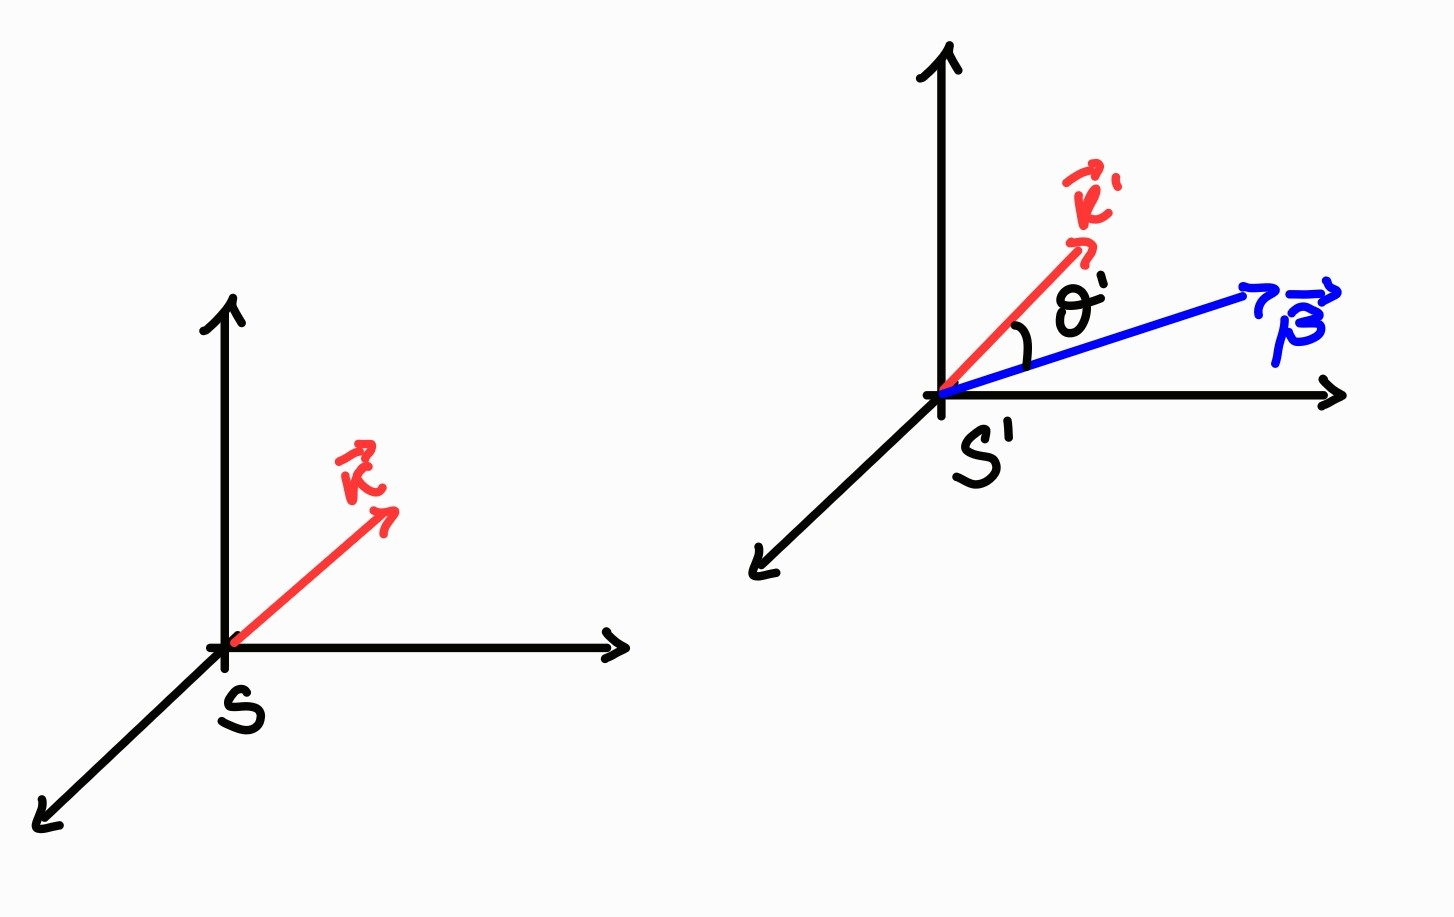
\includegraphics[width=0.40\textwidth]{Immagini/Doppler.jpg}
    \caption{ Sistemi di riferimento inerziali con vettore d'onda}
    \label{fig:Doppler}
\end{figure}

La trasformazione di Lorentz che lega le due quantità è:
\begin{equation}
\begin{gathered}
      k^{\alpha}\xrightarrow[\text{}]{\text{L}}k'^{\beta}=\Lambda\indices{^\beta_\nu}(\Vec{v}) k^{\nu}\\
         k'^{\alpha}\xrightarrow[\text{}]{\text{L}}k^{\beta}=\Lambda\indices{^\beta_\nu}(-\Vec{v}) k'^{\nu}
\end{gathered}
\end{equation}
in particolare sviluppiamo la componente temporale:
\begin{equation}
   \begin{split}
       k^0=\Lambda\indices{^0_\beta} k'^{\beta}=\Lambda\indices{^0_0} k'^{0}+\Lambda\indices{^0_i} k'^{i}=\gamma k'^{0}+\beta_i\gamma k'^{i}&=\gamma[ k'^{0}+\beta_i k'^{i}]=\gamma[ k'^{0}+\Vec{\beta}\Vec{k}']\\
       &=\gamma[ k'^{0}+|\Vec{\beta}||\Vec{k}'|\cos{\theta'}]=\gamma k'^{0}[ 1+|\Vec{\beta}|\cos{\theta'}]
   \end{split}
\end{equation}
ricordando $k^0=|\Vec{k}|=\dfrac{\omega}{c}$ e definendo la frequenza come $\nu=\dfrac{\omega}{2\pi}$ otteniamo:
\begin{equation}\phantomsection\label{eq:Doppler_fre}
       \dfrac{\omega}{c}=\gamma\dfrac{\omega'}{c}[ 1+|\Vec{\beta}|\cos{\theta'}] \implies  \nu=\gamma\nu'[ 1+|\Vec{\beta}|\cos{\theta'}]=\nu'\dfrac{1+|\Vec{\beta}|\cos{\theta'}}{\sqrt{1-\beta^2}}
\end{equation}

Studiamo, ora, il caso particolare nel quale $\Vec{\beta}\parallel\Vec{x}$ e consideriamo l'onda elettromagnetica la cui direzione di moto forma l'angolo $\theta$ con l'asse $x$ e forma l'angolo $\theta'$ con l'asse $x'$.
\begin{figure}[h]
    \centering
    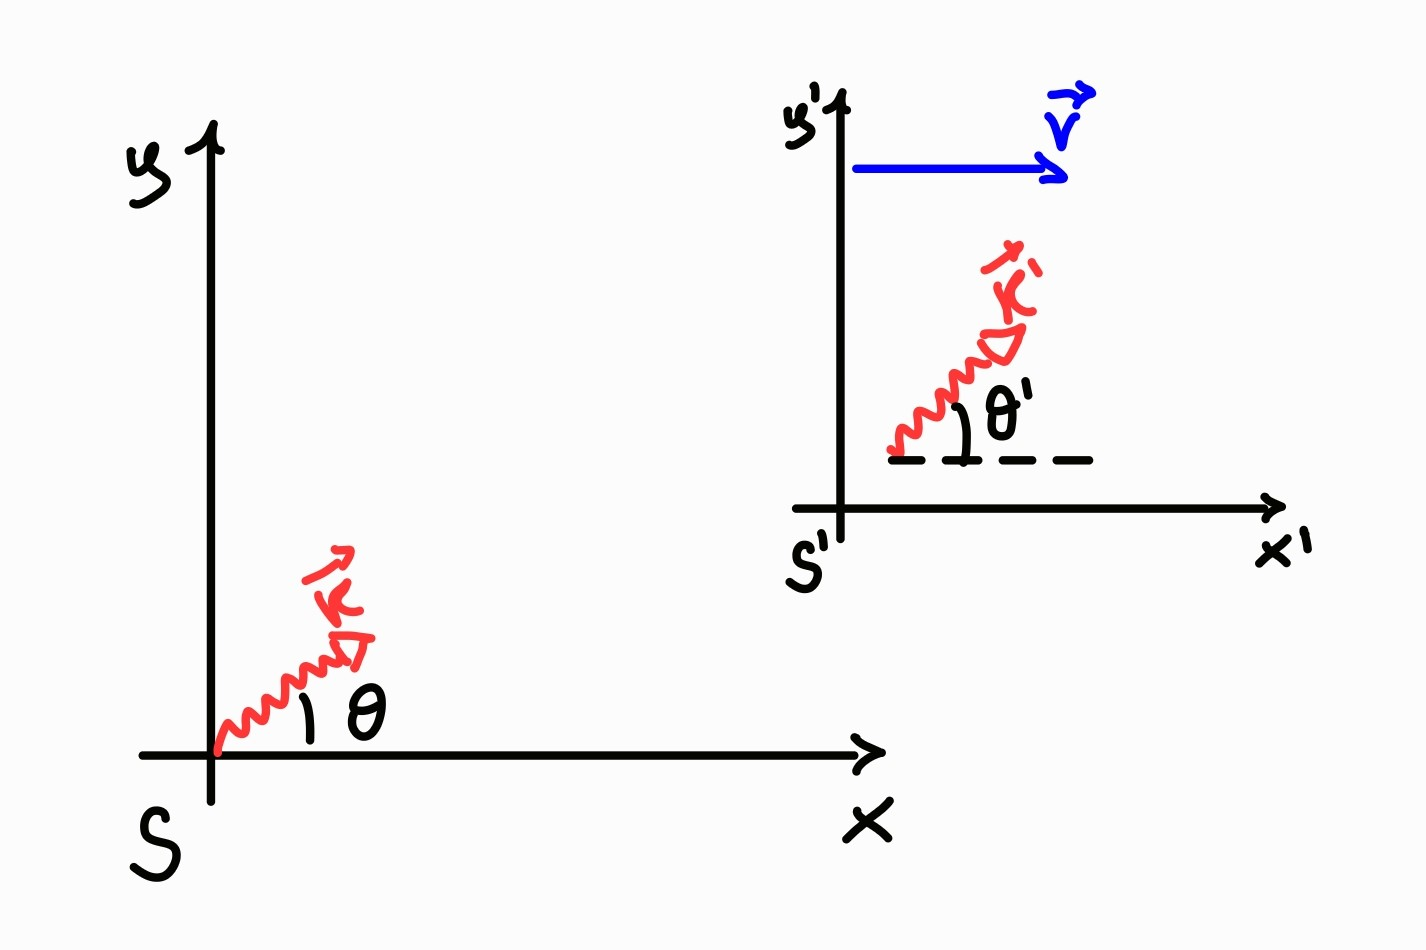
\includegraphics[width=0.40\textwidth]{Immagini/Doppler_unidirezionale .jpg}
    \caption{ Sistemi di riferimento inerziali di moto relativo lungo x e con onda elettromagnetica in direzione arbitraria }
    \label{fig:Doppler_x}
\end{figure}

Invertendo la \eqref{eq:Doppler_fre}, otteniamo:
\begin{equation}
        \nu'=\nu\dfrac{\sqrt{1-\beta^2}}{1+|\Vec{\beta}|\cos{\theta'}}
\end{equation}
studiamo le componenti spaziali x e y del vettore d'onda:
\begin{equation}
   \begin{gathered}
       k^1=\Lambda\indices{^1_\beta} k'^{\beta}=\Lambda\indices{^1_0} k'^{0}+\Lambda\indices{^1_i} k'^{i}=\gamma\beta k'^{0}+\gamma k'^{1}\\
       \implies|\Vec{k}|\cos{\theta}=\gamma k'^{0}[ \beta+\cos{\theta'}]
   \end{gathered}
\end{equation}
esplicito le frequenze sostituendo come prima 
\begin{equation}
     \nu\cos{\theta}=\nu'\dfrac{\beta+\cos{\theta'}}{\sqrt{1-\beta^2}}
\end{equation}
la componete y sarà:
\begin{equation}
   \begin{gathered}
       k^2=\Lambda\indices{^2_\beta} k'^{\beta}=\Lambda\indices{^2_0} k'^{0}+\Lambda\indices{^2_i} k'^{i}= k'^{2}\\
       \implies|\Vec{k}|\sin{\theta}=|\Vec{k}'|\sin{\theta'}\implies \nu\sin{\theta}=\nu'\sin{\theta'}
   \end{gathered}
\end{equation}
concludiamo che si modifica la componente longitudinale al moto, ma non quella trasversale. Determiniamo la relazione che lega i due angoli:
\begin{equation}
     \tan{\theta}=\dfrac{\sin{\theta'}\sqrt{1-\beta^2}}{\cos{\theta'}+\beta}
\end{equation}
Concludiamo questa parte studiando due casi notevoli. Chiamiamo \textit{effetto doppler longitudinale} il caso in cui $\theta'=\theta=0$
\begin{equation}
    \nu=\nu'\dfrac{1+|\Vec{\beta}|\cos{\theta'}}{\sqrt{1-\beta^2}}=\nu'\dfrac{\sqrt{1+\beta}}{\sqrt{1-\beta}}
\end{equation}
 invece, chiamiamo \textit{effetto doppler trasverso} il caso in cui $\theta'=\dfrac{\pi}{2}$
\begin{equation}
    \nu=\nu'\dfrac{1+|\Vec{\beta}|\cos{\theta'}}{\sqrt{1-\beta^2}}=\nu'\dfrac{1}{\sqrt{1-\beta^2}}
\end{equation}
possiamo notare che il primo termine correttivo nell'effetto doppler trasverso è del secondo ordine in $\beta$, questo significa che sperimentalmente risulta più difficile, rispetto all'effetto doppler longitudinale, da misurare.

\subsection{Soluzione con sorgenti}
Consideriamo le equazioni di Maxwell con la condizione di gauge di Lorentz \eqref{eq:Max_gauge} nel caso generale in cui siano presenti sorgenti:
\begin{equation}
\begin{cases}\phantomsection\label{eq:Maxwell_sorgenti}
  \Box A^\nu(t,\Vec{x})=\dfrac{4\pi}{c}j^\nu(t,\Vec{x})\\
  \partial_\mu A^\mu=0
\end{cases}
\end{equation}
la soluzione sarà data dalla somma di una parte omogenea, già discussa in sezione \ref{sec:2.7}, e di una parte particolare. Il metodo che utilizzeremo è detto delle funzioni di Green.

Introduciamo una \textit{funzione di Green} come una funzione biscalare\footnote{Ossia uno scalare che dipende da due eventi.} $D(t,\Vec{x};t',\Vec{x}')$ che soddisfa la relazione:
\begin{equation}\phantomsection\label{eq:Def_Green}
    \Box_x D(t,\Vec{x};t',\Vec{x}')=\delta^4(x-x')=\delta(ct-ct')\delta^3(\Vec{x}-\Vec{x}')
\end{equation}
specifichiamo che il pedice all'operatore dalembertiano indica che quest'ultimo agisce sulle coordinate non primate. Dimostriamo rapidamente che l'oggetto appena introdotto è uno scalare.
\begin{proof}
    Dalla proprietà della delta sappiamo
    \begin{equation}
        \int d^4xf(x)\delta^4(x-y)=f(y)
    \end{equation}
    in particolare se poniamo $f(x)=1$
     \begin{equation}
        \int d^4x\delta^4(x)=1
    \end{equation}
    concludiamo che essendo la misura uno scalare e il risultato dell'integrazione anche, ne consegue necessariamente che la $\delta^4(x)$ sarà uno scalare e, dalla definizione, lo sarà anche $D(t,\Vec{x};t',\Vec{x}')$.
    \end{proof}
Poiché lo spazio di Minkowski è omogeneo, la funzione di Green deve essere invariante per traslazioni, quindi la sua dipendenza non sarà definita dai due eventi separatamente, bensì dalla loro differenza. Pertanto possiamo riscrivere la dipendenza come:
\begin{equation}
   D(t-t',\Vec{x}-\Vec{x}')=D(x-x')
\end{equation}
quindi possiamo riscrivere anche la definizione della funzione di Green, come:
\begin{equation}
    \Box_x D(x-x')=\delta^4(x-x')
\end{equation}
Si può dimostrare, e lo faremo subito, che una soluzione particolare della \eqref{eq:Maxwell_sorgenti} è:

\begin{equation}\phantomsection\label{eq:Maxwell_sorgenti_sol}
  A^\alpha(t,\Vec{x})=\dfrac{4\pi}{c}\int d^4x'D(x-x')j^\alpha(t',\Vec{x}')\footnote{Possiamo notare che in questa forma il potenziale ha l'aspetto di un prodotto di convoluzione: \\$(f*g)(x)=\int_{\mathbb{R}^n}f(x-y)g(y)dy$.}
\end{equation}
applicando l'operatore di D'Alembert, otteniamo:\begin{equation}
  \Box_x A^\alpha(t,\Vec{x})=\dfrac{4\pi}{c}\int d^4x'\Box_xD(x-x')j^\alpha(t',\Vec{x}')=\dfrac{4\pi}{c}\int d^4x'\delta^4(x-x')j^\alpha(t',\Vec{x}')=\dfrac{4\pi}{c}j^\alpha(t,\Vec{x})
\end{equation}
la delta di Dirac ha supporto solo quando i due eventi coincidono, quindi l'integrale si riduce all'equazione iniziale. Concludiamo che conoscendo una funzione di Green, in linea di principio, grazie alla \eqref{eq:Maxwell_sorgenti_sol}, abbiamo una soluzione. A questo punto dobbiamo determinare una forma analitica per la funzione di Green, per farlo procederemo utilizzando la trasformata di Fourier\footnote{ Difatti, spesso, per risolvere equazioni differenziali si fa uso delle trasformate di Fourier, questo perché un'equazione differenziale, nello spazio iniziale, diventa una semplice equazione algebrica, nello spazio di Fourier.}.

Rappresentiamo, quindi, la funzione di Green con una trasformata di Fourier quadridimensionale:
\begin{equation}\phantomsection\label{eq:Green_Fourier}
  D(x-x')=\dfrac{1}{(2\pi)^4}\int d^4k\quad e^{-ik_\alpha(x^\alpha-x'^\alpha)} \Tilde{D}(k)
\end{equation}
mentre la rappresentazione della delta di Dirac è:
\begin{equation}\phantomsection\label{eq:Dirac_Fourier}
  \delta^4(x-x')=\dfrac{1}{(2\pi)^4}\int d^4k\quad e^{-ik_\alpha(x^\alpha-x'^\alpha)} 
\end{equation}
Dunque la definizione della funzione di Green \eqref{eq:Def_Green} diventa, in termini delle rappresentazioni di Fourier:
\begin{equation}
\begin{gathered}
        \Box_x D(x-x')=\delta^4(x-x')\\  \Box_x \dfrac{1}{(2\pi)^4}\int d^4k\quad e^{-ik_\alpha(x^\alpha-x'^\alpha)} \Tilde{D}(k)=\dfrac{1}{(2\pi)^4}\int d^4k\quad e^{-ik_\alpha(x^\alpha-x'^\alpha)} \\
        \dfrac{1}{(2\pi)^4}\int d^4k\quad (-k_\mu k^\mu)e^{-ik_\alpha(x^\alpha-x'^\alpha)} \Tilde{D}(k)=\dfrac{1}{(2\pi)^4}\int d^4k\quad e^{-ik_\alpha(x^\alpha-x'^\alpha)}
\end{gathered}
\end{equation}
ove ricordiamo che $\Box_x=\partial_\mu\partial^\mu$ e l'unico termine che dipende da $x$ è l'esponenziale. Inoltre, per la completezza delle funzioni nello spazio di Fourier possiamo scrivere:\begin{equation}
-k_\mu k^\mu \Tilde{D}(k)=1 \implies \Tilde{D}(k)=-\dfrac{1}{k_\mu k^\mu}=-\dfrac{1}{(k_0)^2 -|\Vec{k}|^2}
\end{equation}
ottenendo, così, un equazione algebrica. Per semplificare la notazione consideriamo $|\Vec{k}|^2=k^2$. 

Sostituendo quanto appena ottenuto nella \eqref{eq:Green_Fourier}:
\begin{equation}\phantomsection\label{eq:int_green}
\begin{split}
     D(x-x')&=\dfrac{1}{(2\pi)^4}\int d^4k\quad e^{-ik_\alpha(x^\alpha-x'^\alpha)}\dfrac{1}{k^2-k\indices{_0^2}}\\
     &=\dfrac{1}{(2\pi)^4}\int d^3k\quad e^{i\Vec{k}(\Vec{x}-\Vec{x}')}\int^{\infty}_{-\infty} dk_0\quad e^{-ik_0(ct-ct')}\dfrac{1}{k^2-k\indices{_0^2}}
\end{split}
\end{equation}

si pone il problema di scegliere una funzione di Green tra le infinite possibili.
Per ragioni fisiche di causalità richiediamo che la funzione di Green soddisfi la \textit{condizione di ritardo}, ossia:
\begin{equation}
    D(x-x')=0 \qquad \forall t<t'
\end{equation}
fisicamente tale condizione significa che la funzione di Green non dipende da eventi che siano temporalmente successivi a quello dell'osservatore. 

Ora, dobbiamo risolvere l'integrale \eqref{eq:int_green}, notiamo che presenta due poli sul percorso di integrazione. 
\begin{equation}
    k^2-k\indices{_0^2}=(k+k_0)(k-k_0)
\end{equation}
Per risolverlo pensiamo, momentaneamente, a $k_0$ come complesso e facciamo la prescrizione che consiste nella sottrazione di una parte immaginaria tendente a zero, cosicché il percorso sia integrabile.
\begin{equation}
    k^2-k\indices{_0^2}=(k+k_0)(k-k_0)=\lim_{\epsilon\to0^+} (k+i\epsilon+k_0)(k-i\epsilon-k_0)
\end{equation}
\begin{figure}[H]
    \centering
    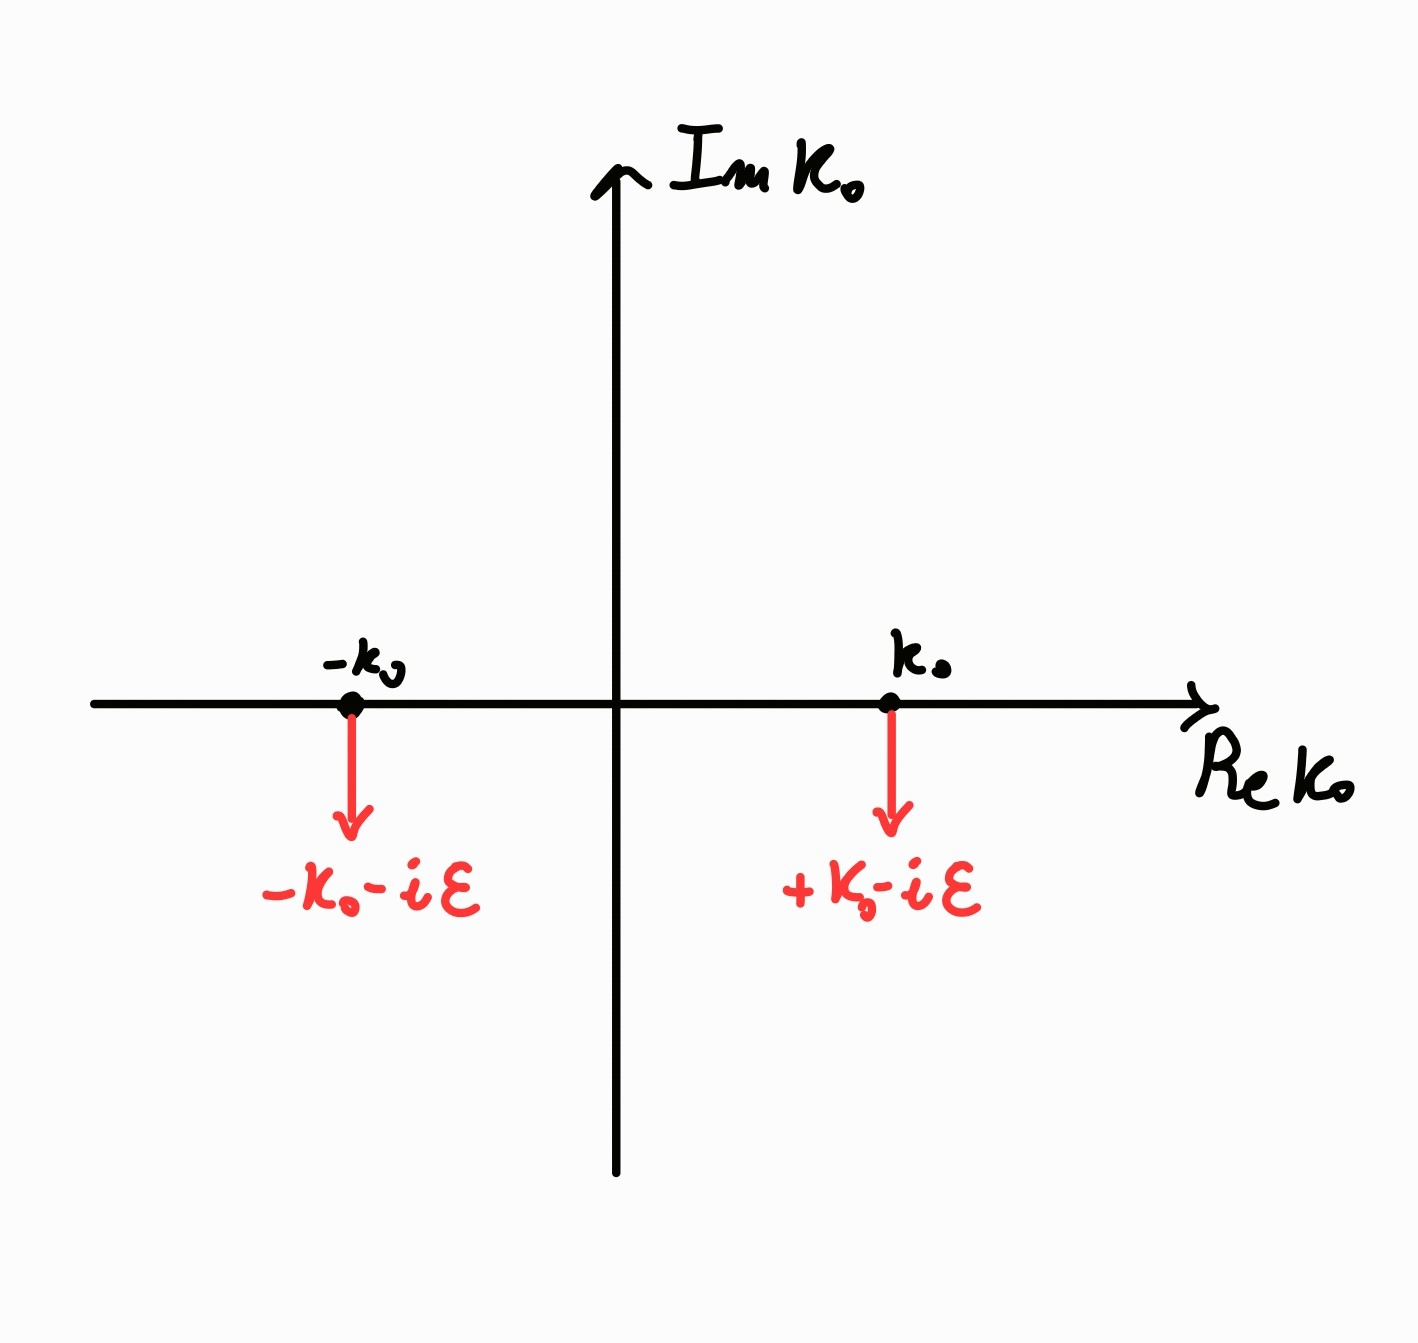
\includegraphics[width=0.40\textwidth]{Immagini/Prescrizione.jpg}
    \caption{Spostamento dei punti singolari al di sotto della retta reale di integrazione.}
    \label{fig:prescrizione}
\end{figure}

Definiamo l'integrale sul piano complesso di $k_0$
\begin{equation}\phantomsection\label{eq:int_compl}
J_{ret}(k)=\lim_{\epsilon\to0^+} \int^{\infty}_{-\infty} dk_0\quad \dfrac{e^{-ick_0(t-t')}}{(k+i\epsilon+k_0)(k-i\epsilon-k_0)}
\end{equation}
\begin{figure}[H]
    \centering
    \subfloat[\centering Integrazione semipiano superiore.]{{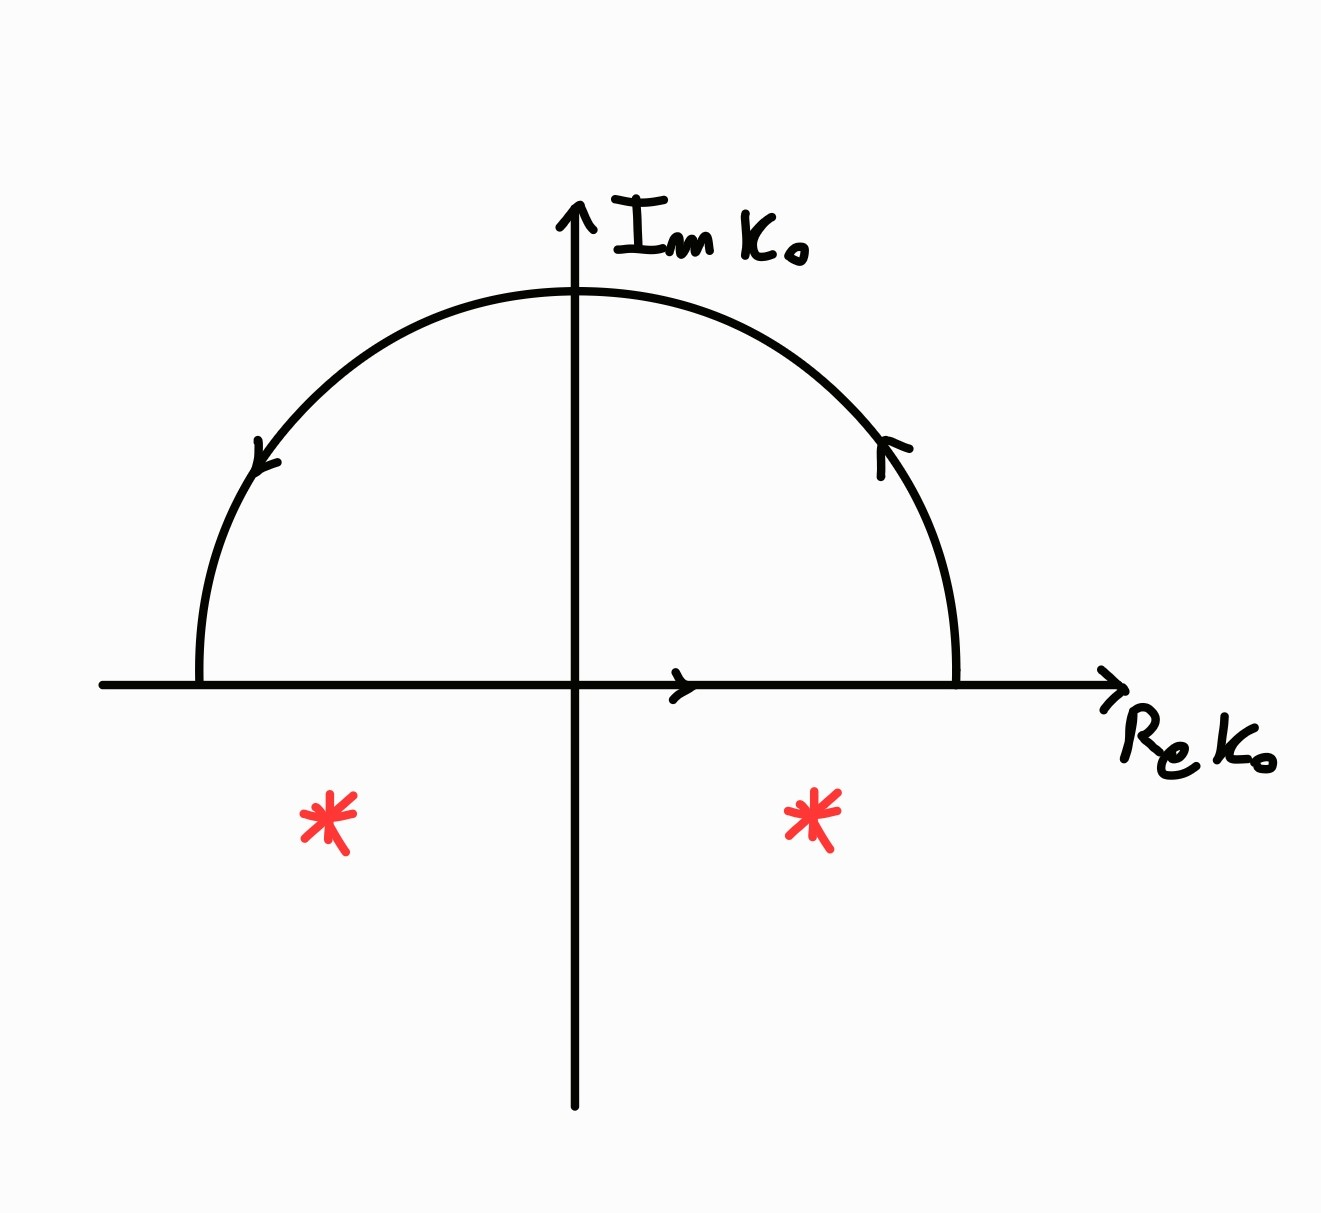
\includegraphics[width=5cm]{Immagini/Residuo_sup.jpg} }}%
    \qquad
    \subfloat[\centering Integrazione semipiano inferiore.]{{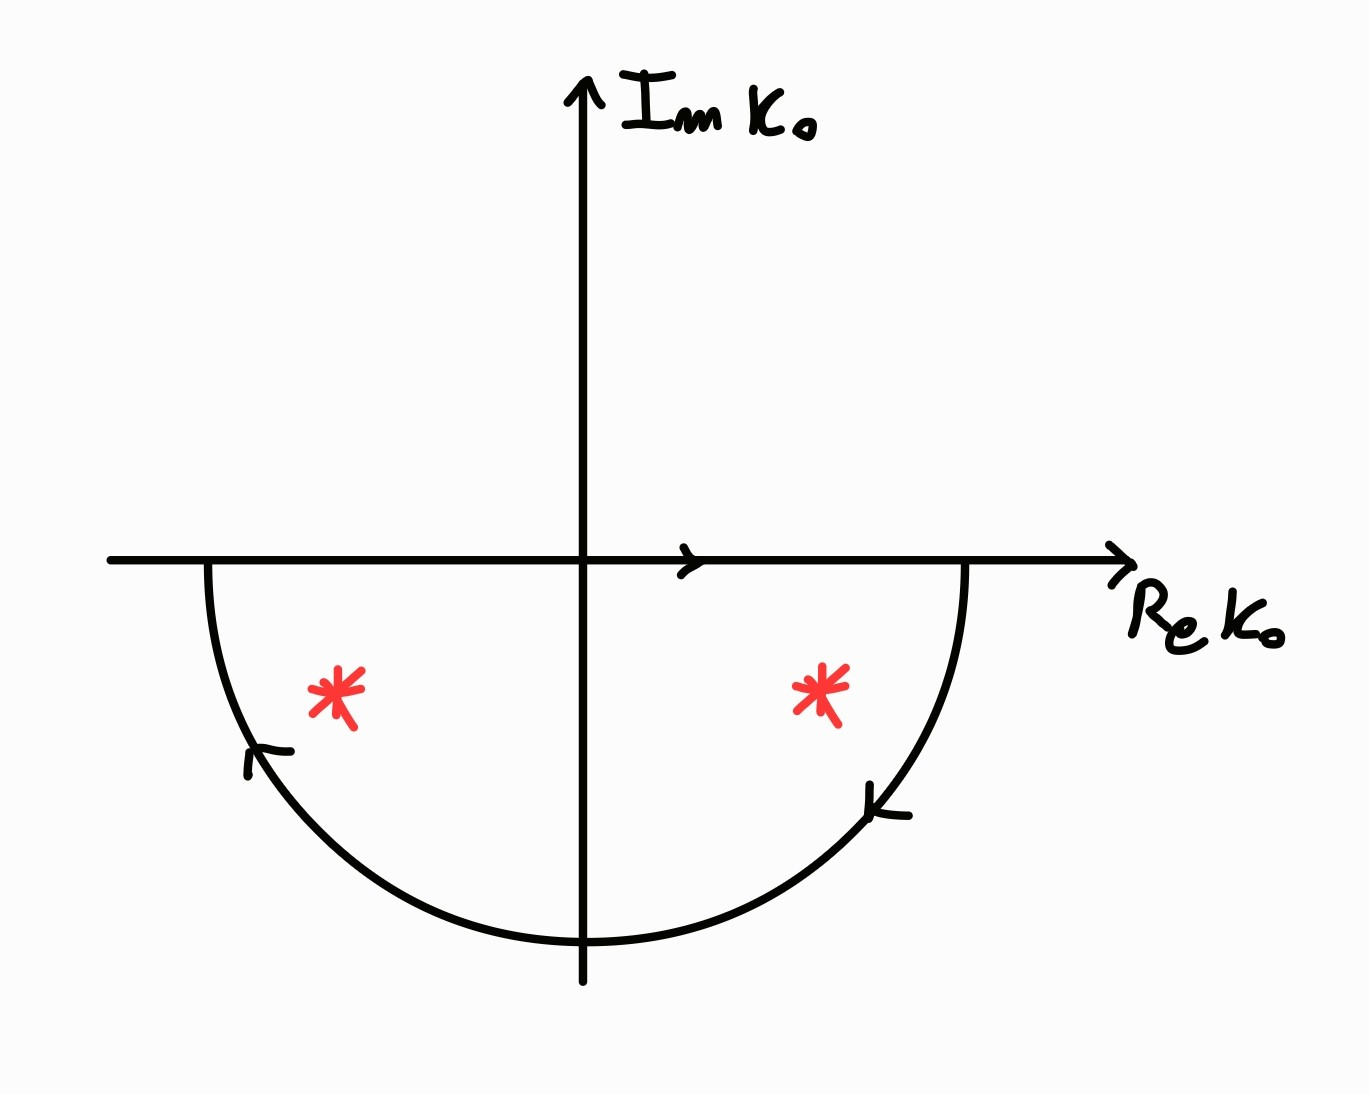
\includegraphics[width=5cm]{Immagini/Residuo_inf.jpg} }}%
    \caption{Integrazione nel piano complesso.}%
    \label{fig:Residuo}%
\end{figure}
Per risolvere l'integrale \eqref{eq:int_compl} consideriamo i percorsi rappresentati in Fig.\ref{fig:Residuo}. In particolare, per $t<t'$ abbiamo che la funzione integranda è analitica nel semipiano superiore, quindi, per il lemma di Jordan, il risultato dell'integrazione è nullo.
Mentre per $t>t'$ la funzione è sempre analitica ed applicando il teorema dei residui, avendo due poli semplici, otteniamo:
 \begin{equation}
J_{ret}(k)=-2\pi i \dfrac{e^{ick(t-t')}-e^{-ick(t-t')}}{2k}\Theta(ct-ct')
\end{equation}
ove la funzione $\Theta(ct-ct')$ non è altro che una funzione a gradino che vale $0$ per $t<t'$ e $1$ per $t>t'$\footnote{Questa ci serve unicamente per ricordarci della condizione di ritardo.}.
Possiamo manipolare il risultato ottenuto
 \begin{equation}
 \begin{aligned}
      J_{ret}(k)&=-2\pi i \dfrac{e^{ick(t-t')}-e^{-ick(t-t')}}{2k}\Theta(ct-ct')=  2\pi\dfrac{e^{ick(t-t')}-e^{-ick(t-t')}}{2ki}\Theta(ct-ct')\\
      &=2\pi\dfrac{\sin{[ck(t-t')]}}{k}\Theta(ct-ct')
 \end{aligned}
\end{equation}
Sostituendolo nella \eqref{eq:int_green} otteniamo la Funzione di Green ritardata:
\begin{equation}
   \begin{aligned}
        D_{ret}(x-x')&=\dfrac{1}{(2\pi)^4}\int d^3k\quad e^{i\Vec{k}(\Vec{x}-\Vec{x}')}2\pi\dfrac{\sin{[ck(t-t')]}}{k}\Theta(ct-ct')\\
     &=\dfrac{1}{(2\pi)^3}\int d^3k\quad e^{i\Vec{k}(\Vec{x}-\Vec{x}')}\dfrac{\sin{[ck(t-t')]}}{k}\Theta(ct-ct')
   \end{aligned}
\end{equation}
Ci rimane solamente da risolvere l'integrale, per farlo definiamo $\Vec{R}=\Vec{x}-\Vec{x}'$ ed in particolare scegliamo\footnote{Possiamo farlo perché, nello spazio di Minkowki, abbiamo l'invarianza per rotazioni.} $\Vec{x}-\Vec{x}'\parallel \Vec{z}$. Inoltre consideriamo il prodotto $\Vec{k}(\Vec{x}-\Vec{x}')=kR\cos{\theta}$, ove $\theta$, per la scelta di prima, è l'angolo azimutale. A questo punto passiamo in coordinate sferiche\footnote{Ricordiamo che la misura cambia in $d^3k=k^2dk\sin{\theta}d\theta d\phi$.} e riscriviamo l'integrale.
\begin{equation}\phantomsection\label{eq:ret_green}
   \begin{aligned}
        D_{ret}(x-x')&=\dfrac{1}{(2\pi)^3}\int k^2dk\sin{\theta}d\theta d\phi \quad e^{ikR\cos{\theta}}\dfrac{\sin{[ck(t-t')]}}{k}\Theta(ct-ct')\\
        &=\dfrac{1}{(2\pi)^3}\int_0^\infty kdk\sin{[ck(t-t')]}\int_0^\pi d\theta \sin{\theta}e^{ikR\cos{\theta}} \int_0^{2\pi}d\phi \quad\Theta(ct-ct')\\
        &=\dfrac{1}{(2\pi)^2}\int_0^\infty kdk\sin{[ck(t-t')]}\int_0^\pi d\theta \sin{\theta}e^{ikR\cos{\theta}}  \quad\Theta(ct-ct')
   \end{aligned}
\end{equation}
Consideriamo il cambio di variabile $\xi=\cos{\theta}$, da cui $d\theta=-\dfrac{d\xi}{\sin{\theta}}$
\begin{equation}
   \begin{aligned}
        D_{ret}(x-x')&=\dfrac{1}{(2\pi)^2}\int_0^\infty kdk\sin{[ck(t-t')]}\int_0^\pi d\theta \sin{\theta}e^{ikR\cos{\theta}}  \quad\Theta(ct-ct')\\
        &=\dfrac{1}{(2\pi)^2}\int_0^\infty kdk\sin{[ck(t-t')]}\int_{-1}^1 d\xi e^{ikR\xi}  \quad\Theta(ct-ct')\\
        &=\dfrac{1}{(2\pi)^2}\int_0^\infty kdk\sin{[ck(t-t')]} \dfrac{e^{ikR}-e^{-ikR}}{ikR}  \quad\Theta(ct-ct')\\
         &=\dfrac{1}{(2\pi)^2}\int_0^\infty dk\sin{[ck(t-t')]} \dfrac{e^{ikR}-e^{-ikR}}{iR} \dfrac{2}{2} \quad\Theta(ct-ct')\\
          &=\dfrac{2}{(2\pi)^2R}\int_0^\infty dk\sin{[ck(t-t')]} \sin{kR}  \quad\Theta(ct-ct')\\
   \end{aligned}
\end{equation}
la funzione integranda, così ottenuta, è ovviamente pari poiché prodotto di funzioni dispari
\begin{equation}
   \begin{aligned}
        D_{ret}(x-x')&=\dfrac{1}{(2\pi)^2R}\int_{-\infty}^\infty dk\sin{[ck(t-t')]} \sin{kR}  \quad\Theta(ct-ct')\\
        &=\dfrac{1}{(2\pi)^2R}\left(-\dfrac{1}{4}\right)\int_{-\infty}^\infty dk [e^{ick(t-t')}-e^{-ick(t-t')}][e^{ikR}-e^{-ikR}]  \quad\Theta(ct-ct')\\
        &=\dfrac{1}{4(2\pi)^2R}\int_{-\infty}^\infty dk [e^{-ick(t-t')}-e^{ick(t-t')}][e^{ikR}-e^{-ikR}]  \quad\Theta(ct-ct')\\
         &=\dfrac{1}{4(2\pi)^2R}\int_{-\infty}^\infty dk \{e^{-ik[c(t-t')-R]}-e^{-ik[c(t-t')+R]}\\&\qquad \qquad\qquad\qquad\quad-e^{ik[c(t-t')+R]}+e^{ik[c(t-t')-R]} \}\Theta(ct-ct')\\
   \end{aligned}
\end{equation}
Ora, ricordando la \eqref{eq:Dirac_Fourier}, per una sola dimensione, e ricordando la proprietà $\delta(x)=\delta(-x)$
\begin{equation}
   \begin{aligned}
        D_{ret}(x-x')=\dfrac{2\pi}{4(2\pi)^2R}&\{ \delta[c(t-t')-R]-\delta[c(t-t')+R]\\
       & -\delta[c(t-t')+R]+\delta[c(t-t')-R] \}\Theta(ct-ct')\\
   \end{aligned}
\end{equation}
quello che sappiamo è che la delta ha supporto solo quando il suo argomento è nullo. Analizziamo gli argomenti: la sottrazione $t-t'$ è positiva sotto la garanzia della funzione $\Theta(ct-ct')$ e $R=|\Vec{x}-\Vec{x}'|$ è positiva per definizione. Quindi gli argomenti delle delta nelle quali i fattori sono sommati non si annulleranno mai, dunque, ha senso tenere solo $\delta[c(t-t')-R]$:
\begin{equation}\phantomsection\label{eq:Green_ret}
        D_{ret}(x-x')=\dfrac{2}{4(2\pi)R}\delta[c(t-t')-R]\Theta(ct-ct')=\dfrac{1}{4\pi}\dfrac{\delta[c(t-t')-R]}{|\Vec{x}-\Vec{x}'|}\Theta(ct-ct')
\end{equation}
questa è la funzione di Green ritardata per l'operatore di D'Alembert.

Sostituendola nella \eqref{eq:Maxwell_sorgenti_sol}
\begin{equation}
  A_{ret}^\alpha(t,\Vec{x})=\dfrac{4\pi}{c}\int d^4x'D(x-x')j^\alpha(t',\Vec{x}')=\dfrac{1}{c}\int d(ct')d^3x'\dfrac{\delta[c(t-t')-|\Vec{x}-\Vec{x}'|]}{|\Vec{x}-\Vec{x}'|}j^\alpha(t',\Vec{x}')
\end{equation}
ci rimane da calcolare questo integrale. L'integrazione in $t'$ è immediata, poiché la delta avrà supporto solo per 
\begin{equation}\phantomsection\label{eq:t_ret}
    c(t-t')=|\Vec{x}-\Vec{x}'| \implies t'=t-\dfrac{|\Vec{x}-\Vec{x}'|}{c}
\end{equation}
quindi l'unico contributo dell'integrazione sarà dato da $t'$:
\begin{equation}\phantomsection\label{eq:soluz_rita}
  A_{ret}^\alpha(t,\Vec{x})=\int d^3x'\dfrac{j^\alpha(t-\dfrac{R}{c},\Vec{x}')]}{|\Vec{x}-\Vec{x}'|}
\end{equation}
\`E doveroso fare alcune osservazioni. Se consideriamo (come mostrato in Fig.\ref{fig:Green}) un osservatore all'evento $P(t,\Vec{x})$ e una carica all'evento $Q=(t',\Vec{x}')$, la relazione \eqref{eq:soluz_rita} descrive il campo percepito dall'osservatore. Il fatto che tale relazione dipenda dalla definizione \eqref{eq:t_ret} del tempo ritardato mostra la causalità intrinseca alla soluzione trovata. Questo significa che ciò che l'osservatore \say{vede} è ristretto a ciò che è contenuto nel suo cono di luce passato\footnote{Viene escluso il cono di luce futuro dalla condizione di ritardo.}, questo perché la radiazione elettromagnetica ha velocità finita.
\begin{figure}[H]
    \centering
    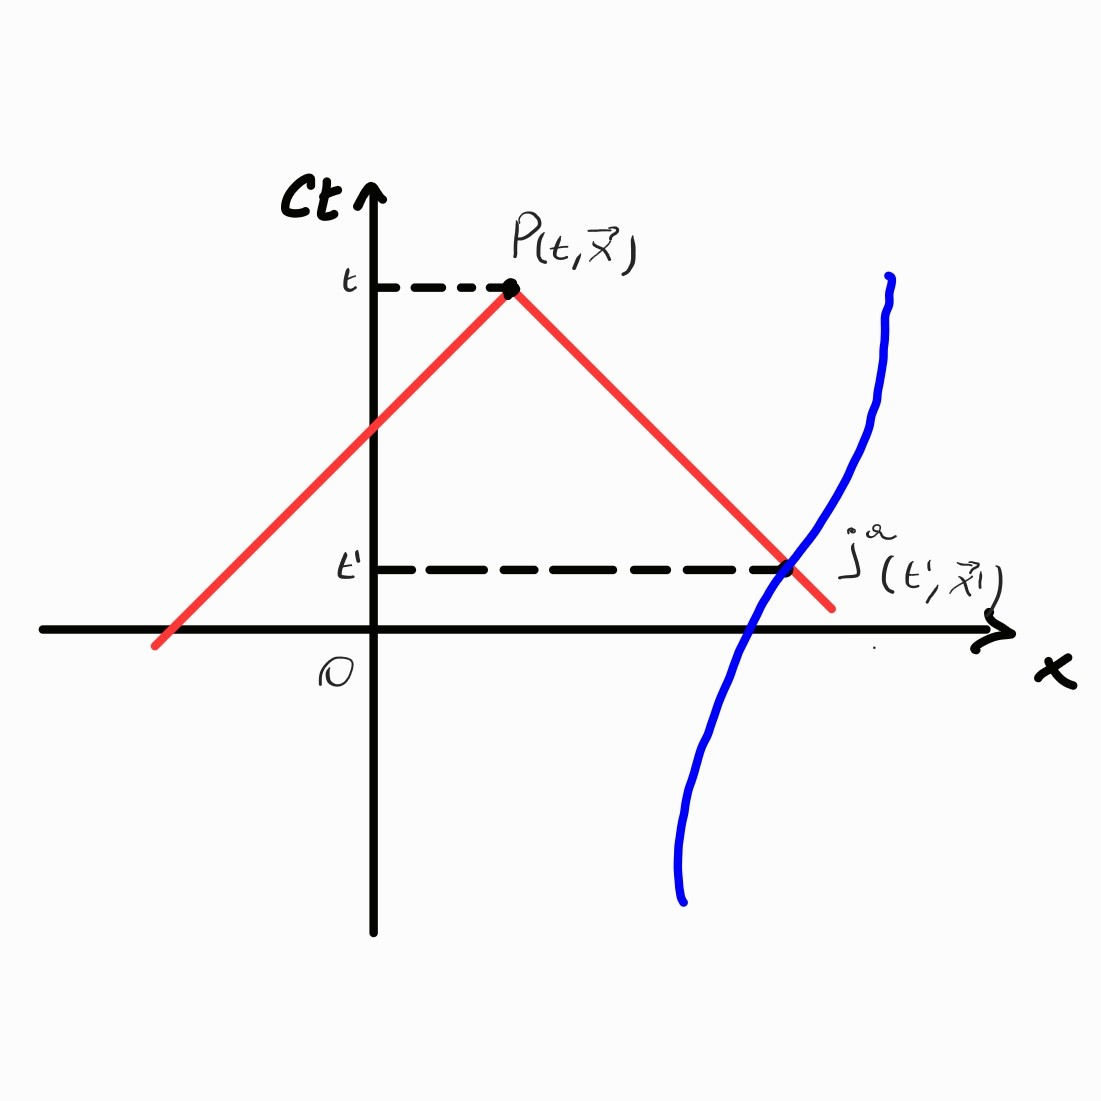
\includegraphics[width=0.35\textwidth]{Immagini/Green.jpg}
    \caption{La rappresentazione grafica di $c=\dfrac{|\Vec{x}-\Vec{x}'|}{t-t'}$ non è altro che il cono di luce.}
    \label{fig:Green}
\end{figure}
Nelle teorie classiche non è così, le velocità sono considerate infinite. Per la teoria gravitazionale di Newton abbiamo che il campo gravitazionale varia istantaneamente secondo l'equazione di Poisson $\nabla^2\phi=4\pi\sigma\rho$.
 
 Ci rimane da mostrare che la funzione di Green sia Lorentz invariante e che soddisfi la condizione di gauge di Lorentz. Per verificare l'invarianza consideriamo gli eventi $x^\alpha=(x^0,\Vec{x})$ e $x'^\alpha=(x'^0,\Vec{x}')$ e definiamo la delta Dirac che sappiamo essere invariante:
 \begin{equation}
 \begin{aligned}
      \delta[(x^\alpha-x'^\alpha)(x_\alpha-x'_\alpha)]&= \delta[(x_0-x'_0)^2-|\Vec{x}-\Vec{x}'|^2]= \delta[(x_0-x'_0)^2-R^2]\\
      &=\delta\{[(x_0-x'_0)+R][(x_0-x'_0)-R]\}
 \end{aligned}
 \end{equation}
 ricordiamo la proprietà $\delta(g(x))=\sum_i \dfrac{\delta(x-x_i)}{|\frac{dg}{dx}|_{x_i}}$ ove $g$ è una funzione tale per cui $g(x_i)=0$, otteniamo:
 \begin{equation}
     \delta[(x^\alpha-x'^\alpha)(x_\alpha-x'_\alpha)]= \dfrac{1}{2R}[\delta(x^0-x'^0+R)+\delta(x^0-x'^0-R)]
 \end{equation}
 se moltiplichiamo la condizione di ritardo possiamo omettere la delta $\delta(x^0-x'^0+R)$ poiché l'argomento non si annulla mai e quindi non ha supporto
  \begin{equation}
  \begin{aligned}
     \delta[(x^\alpha-x'^\alpha)(x_\alpha-x'_\alpha)]\Theta(ct-ct')&= \dfrac{1}{2R}[\delta(x^0-x'^0+R)+\delta(x^0-x'^0-R)]\Theta(ct-ct')\\
     &=\dfrac{1}{2R}[\delta(x^0-x'^0-R)]\Theta(ct-ct')\\
     &\implies \delta(x^0-x'^0-R)=(2R)\delta[(x^\alpha-x'^\alpha)(x_\alpha-x'_\alpha)]
  \end{aligned}
 \end{equation}
 sostituendo nella \eqref{eq:Green_ret} otteniamo:
 \begin{equation}\phantomsection\label{eq:Green_inva}
        D_{ret}(x-x')=\dfrac{1}{4\pi}\dfrac{\delta[c(t-t')-R]}{R}\Theta(ct-ct')=\dfrac{1}{2\pi}\delta[(x^\alpha-x'^\alpha)(x_\alpha-x'_\alpha)]\Theta(ct-ct')
\end{equation}
in questa forma si vede chiaramente che la funzione di Green è uno scalare ed ogni sua parte è Lorentz invariante. Inoltre, la funzione di Green ha supporto solo quando $x\alpha=x'\alpha$ ossia se $x\alpha-x'\alpha$ è un vettore di tipo luce, geometricamente significa che la funzione di Green ha supporto solo sul cono di luce.

Ora dimostriamo che la soluzione trovata \eqref{eq:soluz_rita} soddisfi il gauge di Lorentz, altrimenti il lavoro è sarebbe stato vano.\begin{equation}
  \partial_\alpha A_{ret}^\alpha(t,\Vec{x})=\dfrac{4\pi}{c}\int d^4x'\partial_\alpha D_{ret}(x-x')j^\alpha(x')
\end{equation}
sappiamo che data una funzione che abbia una dipendenza del tipo $F(x-y)$, allora $\dfrac{\partial F}{\partial x}=-\dfrac{\partial F}{\partial y}$. Riscriviamo, dunque, la precedente come:
\begin{equation}
\begin{aligned}
     \partial_\alpha A_{ret}^\alpha&=\dfrac{4\pi}{c}\int d^4x'[-\partial_{\alpha'} D_{ret}(x-x')]j^\alpha(x')=-\dfrac{4\pi}{c}\int d^4x'[\partial_{\alpha'} D_{ret}(x-x')]j^\alpha(x')\\
     &=-\dfrac{4\pi}{c}\left\{\int d^4x'\partial_{\alpha'}[D_{ret}(x-x')j^\alpha(x')]-\int d^4x'D_{ret}(x-x')\partial_{\alpha'}[j^\alpha(x')]\right\}
\end{aligned}
\end{equation}
dall'equazione di continuità \eqref{eq:eq_cont_elett} abbiamo che il secondo integrale ha argomento nullo. Dal teorema di Gauss, in quattro dimensioni, possiamo scrivere:
\begin{equation}
     \partial_\alpha A_{ret}^\alpha=-\dfrac{4\pi}{c}\int d^4x'\partial_{\alpha'}[D_{ret}(x-x')j^\alpha(x')]=-\dfrac{4\pi}{c}\int_\Sigma d\Sigma_\alpha D_{ret}(x-x')j^\alpha(x')
\end{equation}
ove, ovviamente, la superficie $\Sigma$ è una superficie tridimensionale. Ci rimane da dimostrare che tale integrale sia nullo. Per farlo immaginiamo di fissare lo spazio ed espandere il dominio del tempo di integrazione all'infinito, come mostrato in Fig.\ref{fig:Int_inf}. In questo modo, il quadrivettore x-x' è di genere spazio e dunque la funzione di Green è nulla avendo supporto solo quando x-x' è di genere luce. Analogamente, se fissiamo il tempo e andiamo all'infinito spaziale, allora $j^\alpha(x')$ sarà nulla in quanto le cariche sono localizzate entro uno spazio finito, mentre noi stiamo integrando su una superficie tridimensionale che si estende all'infinito (la delta di dirac nella definizione di $j^\alpha(x')$ è sempre nulla).
\begin{figure}[H]
    \centering
    \subfloat[\centering Integrazione temporale.]{{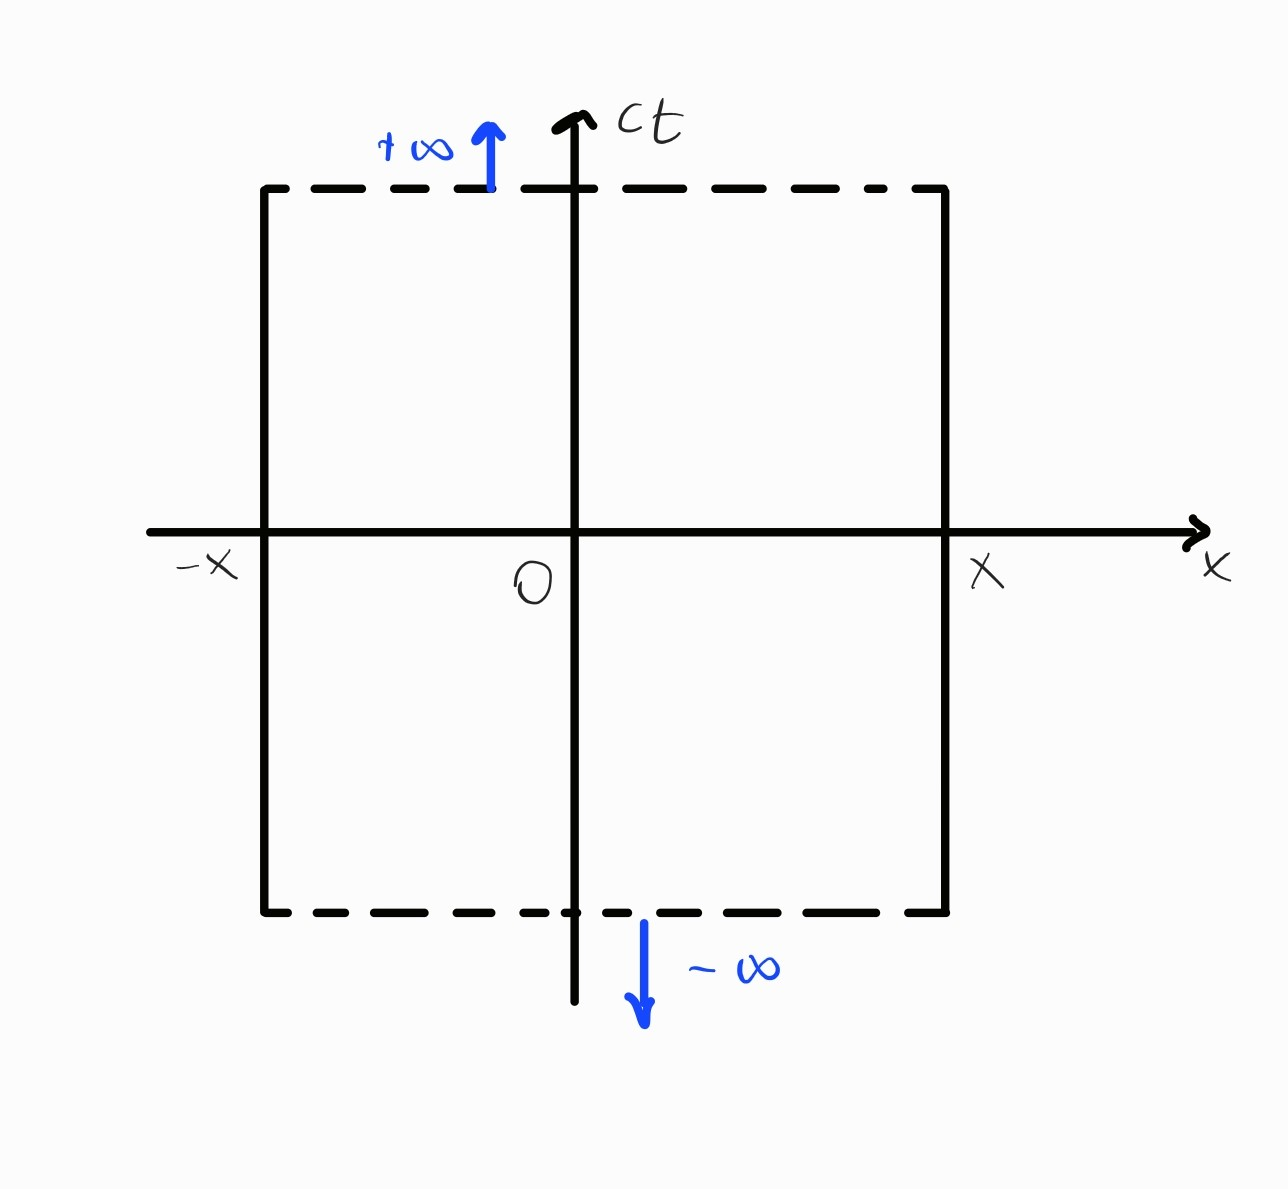
\includegraphics[width=5cm]{Immagini/Integrazione_temporale.jpg} }}%
    \qquad
    \subfloat[\centering Integrazione spaziale.]{{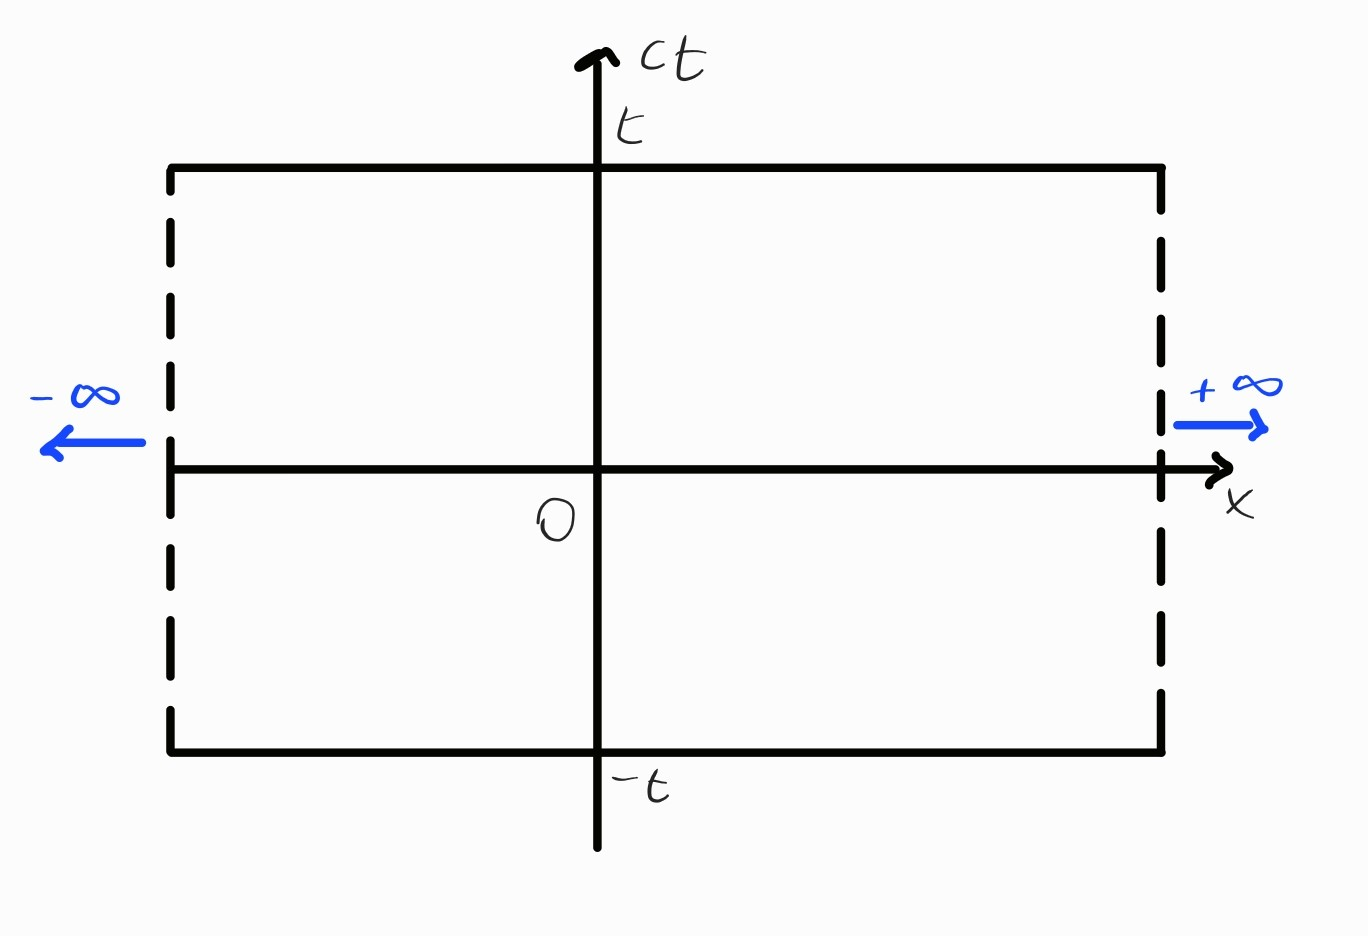
\includegraphics[width=5cm]{Immagini/Integrazione_spaziale.jpg} }}%
    \caption{Integrazione nello spazio di Minkowski.}%
    \label{fig:Int_inf}%
\end{figure}

\subsection{Potenziali di Lienard-Wiechert}
Consideriamo quanto appreso nella sezione \ref{sec:2.2} e applichiamolo al semplice caso di una carica in movimento, al fine di determinarne il potenziale.
Consideriamo la carica $e$ in moto vario lungo la traiettoria $z(t)$, come mostrato in Fig.\ref{fig:Carica}.
\begin{figure}[H]
    \centering
    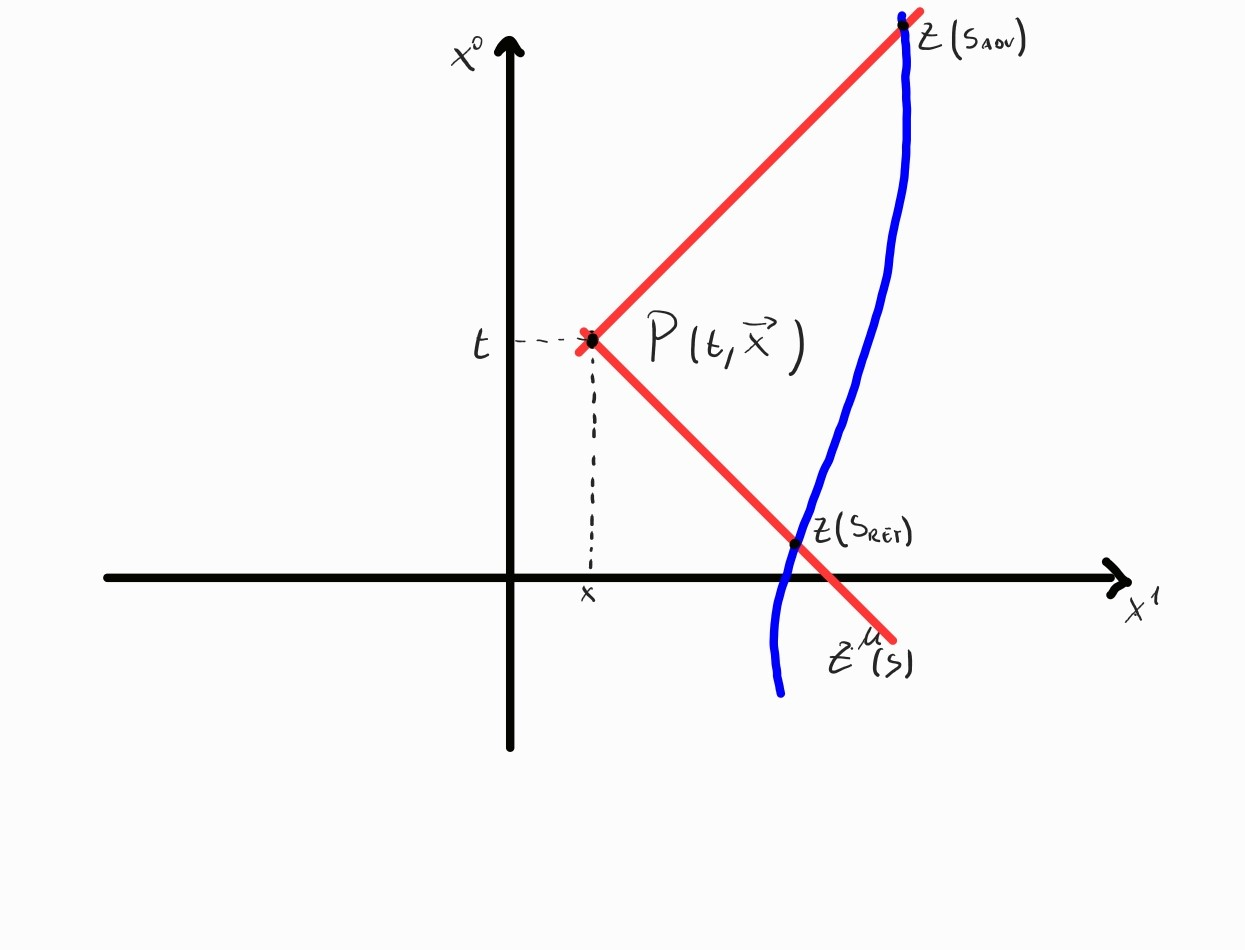
\includegraphics[width=0.36\textwidth]{Immagini/L-W.jpg}
    \caption{Carica in moto vario.}
    \label{fig:Carica}
\end{figure}
Consideriamo, dunque, la \eqref{eq:Maxwell_sorgenti_sol} e sostituiamoci la \eqref{eq:def_quad_corr2} e la \eqref{eq:Green_inva}:
\begin{equation}
\begin{aligned}
     A_{ret}^\alpha(t,\Vec{x})&=\dfrac{4\pi}{c}\int d^4x'D(x-x')j^\alpha(t',\Vec{x}')\\
     &=\dfrac{4\pi}{c}\int d^4x'[\dfrac{1}{2\pi}\delta\left((x-x')^2\right)\Theta(x_0-x'_0)][c\int ds \quad e\delta^4\left(x'-z(s)\right)u^\alpha]\\
     &=2e\iint  d^4x'\quad ds\quad \delta\left((x-x')^2\right)\Theta(x_0-x'_0)\delta^4\left(x'-z(s)\right)u^\alpha
\end{aligned}
\end{equation}
ove la sommatoria delle cariche scompare poiché ne consideriamo una sola. Inoltre, considerando la proprietà della delta $\int dx f(x)\delta(x-y)=f(y)$, quindi sostituiamo ad $x'$ la traiettoria $z(s)$:
\begin{equation}
\begin{aligned}
     A_{ret}^\alpha(t,\Vec{x})&=2e\int ds\quad \delta\left((x-z)^2\right)\Theta(x_0-z_0)u^\alpha(s)\\
     &=2e\int ds\quad \delta\left[(x^0-z^0)^2-|\Vec{x}-\Vec{z}|^2\right]\Theta(x_0-z_0)u^\alpha(s)
\end{aligned}
\end{equation}
ovviamente $x$ rappresenta il punto di osservazione, mentre $z(t)$ la posizione della particella. Perché la delta abbia supporto dobbiamo avere $(x-z)^2=(x_\mu-z_\mu)(x^\mu-z^\mu)=0$, ossia un vettore di tipo luce. Possiamo riscrivere la delta come:
\begin{equation}
     \delta\left[(x^0-z^0)^2-|\Vec{x}-\Vec{z}|^2\right]= \delta\left\{[(x^0-z^0)+|\Vec{x}-\Vec{z}|][(x^0-z^0)-|\Vec{x}-\Vec{z}|]\right\}
\end{equation}
ciò indica due poli, il primo termine rappresenta il polo nel futuro, mentre il secondo rappresenta il polo nel passato, come mostrato in Fig.\ref{fig:Carica}. Per ragioni di causalità, il contributo nel futuro sarà nullo.

Ricordiamo la proprietà $\delta(g(x))=\sum_i \dfrac{\delta(x-x_i)}{|\frac{dg}{dx}|_{x_i}}$, abbiamo che:
\begin{equation}
    \dfrac{d}{ds}\left[(x_\mu-z_\mu)(x^\mu-z^\mu)\right]=-2(x^\mu-z^\mu)\dfrac{dz_\mu}{ds}=-2(x^\mu-z^\mu)u_\mu
\end{equation}
quindi possiamo riscrivere la delta, considerando solo il polo ritardato, come:
\begin{equation}
    \delta\left((x-z)^2\right)\Theta(x_0-z_0)=\dfrac{\delta(s-s_{ret})}{2(x^\mu-z^\mu)u_\mu}
\end{equation}
sostituendolo nel potenziale, otteniamo:\begin{equation}\phantomsection\label{eq:pot_L-W_1}
     A_{ret}^\alpha(t,\Vec{x})=2e\int ds\quad \dfrac{\delta(s-s_{ret})}{2(x^\mu-z^\mu(s))u_\mu}u^\alpha=e\dfrac{u^\alpha}{(x^\mu-z^\mu(s))u_\mu}\biggm|_{s_{ret}}\end{equation}
Però così lo abbiamo espresso nel tempo proprio, vogliamo cambiare parametrizzazione e passare al tempo generico. Sappiamo che $z^\mu(s_{ret})=(ct_{ret},\Vec{z}(t_{ret}))$ e che l'evento generico è $x^\mu=(t,\Vec{x})$, allora:
\begin{equation}
    \begin{gathered}
        (x_\mu-z_\mu)(x^\mu-z^\mu)=0\\
        c^2(t-t_{ret})^2-|\Vec{x}-\Vec{z}|^2=c^2(t-t_{ret})^2-|\Vec{R}|^2=0\\
        \implies t_{ret}=t-\dfrac{R(t_{ret})}{c}
    \end{gathered}
\end{equation}
Ricordando la definizione della quadrivelocità \eqref{eq:def_qvel}, abbiamo che:
\begin{equation}
      (x^\mu-z^\mu)u_\mu=\gamma\left[(ct-ct_{ret})^2-\Vec{R}(t_{ret})\Vec{\beta}(t_{ret})\right]=\gamma(R-\Vec{R}\Vec{\beta})\biggm|_{t_{ret}}
\end{equation}
sostituendolo nella \eqref{eq:pot_L-W_1}, otteniamo le componenti del potenziale:
\begin{equation}\phantomsection\label{eq:pot_L-W_2}
\begin{cases}
     A_{ret}^0(t,\Vec{x})=e\dfrac{u^0}{\gamma(R-\Vec{R}\Vec{\beta})}\biggm|_{t_{ret}}=\dfrac{e}{(R-\Vec{R}\Vec{\beta})}\biggm|_{t_{ret}}
     \\
     \\
     \Vec{A}_{ret}(t,\Vec{x})=\dfrac{e}{c}\dfrac{\Vec{u}}{\gamma(R-\Vec{R}\Vec{\beta})}\biggm|_{t_{ret}}=\dfrac{e}{c^2}\dfrac{\Vec{v}}{(R-\Vec{R}\Vec{\beta})}\biggm|_{t_{ret}}
\end{cases}
\end{equation}
il potenziale trovato è detto \textit{potenziale di Lienard-Wiechert}.

A partire da questo potenziale è possibile ottenere le equazioni del campo elettrico e del campo magnetico generati dalla carica in moto vario. Le riportiamo per completezza, ma non le ricaveremo. Consideriamo il tensore elettromagnetico datoci dal lemma di Poincaré $F\indices{^{\mu\nu}}=\partial^\mu A\nu-\partial^\nu A\mu$, definiamo $\Vec{R}=\Vec{x}-\Vec{z}(t)$ e il versore $\hat{n}=\dfrac{\Vec{R}}{|\Vec{R}|}$, allora il campo elettrico è dato da:
\begin{equation}
    \Vec{E}(t,\Vec{x})=e\left\{\dfrac{(1-\beta^2)(\hat{n}-\Vec{\beta})}{R^2(1-\Vec{\beta}\hat{n})^3} \right\}_{ret}+\dfrac{e}{c}\left\{\dfrac{\hat{n}\times[(\hat{n}-\beta^2)\times \Vec{\dot{\beta}}]}{R^2(1-\Vec{\beta}\hat{n})^3} \right\}_{ret}
\end{equation}
osserviamo che il primo termine dipende solo dalla velocità, quindi descrive il campo per la particella in moto rettilineo uniforme, il secondo termine dipende anche dall'accelerazione, quindi compare se il moto è accelerato, inoltre è il responsabile dell'irraggiamento.

Mentre il campo magnetico segue da:
\begin{equation}
    \Vec{B}(t,\Vec{x})=\left(\hat{n}\times\Vec{E}\right)_{ret}
\end{equation}